\chapter{Комбинирование наборов данных}
\section{Использование соединений}

\subsection{Перекрестные соединения CROSS JOIN}
Это соединение выполняет то, что называют
декартовым произведением двух входных таблиц


\begin{lstlisting}[label=lst:funcReturn, caption=Пример CROSS JOIN, language=sql]
SELECT D.n AS theday, S.n AS shiftno
FROM dbo.Nums AS D
	CROSS JOIN dbo.Nums AS S
WHERE D.n <= 7
	AND S.N <= 3
ORDER BY theday, shiftno;
\end{lstlisting}

\begin{figure}[h!]
	\begin{center}
		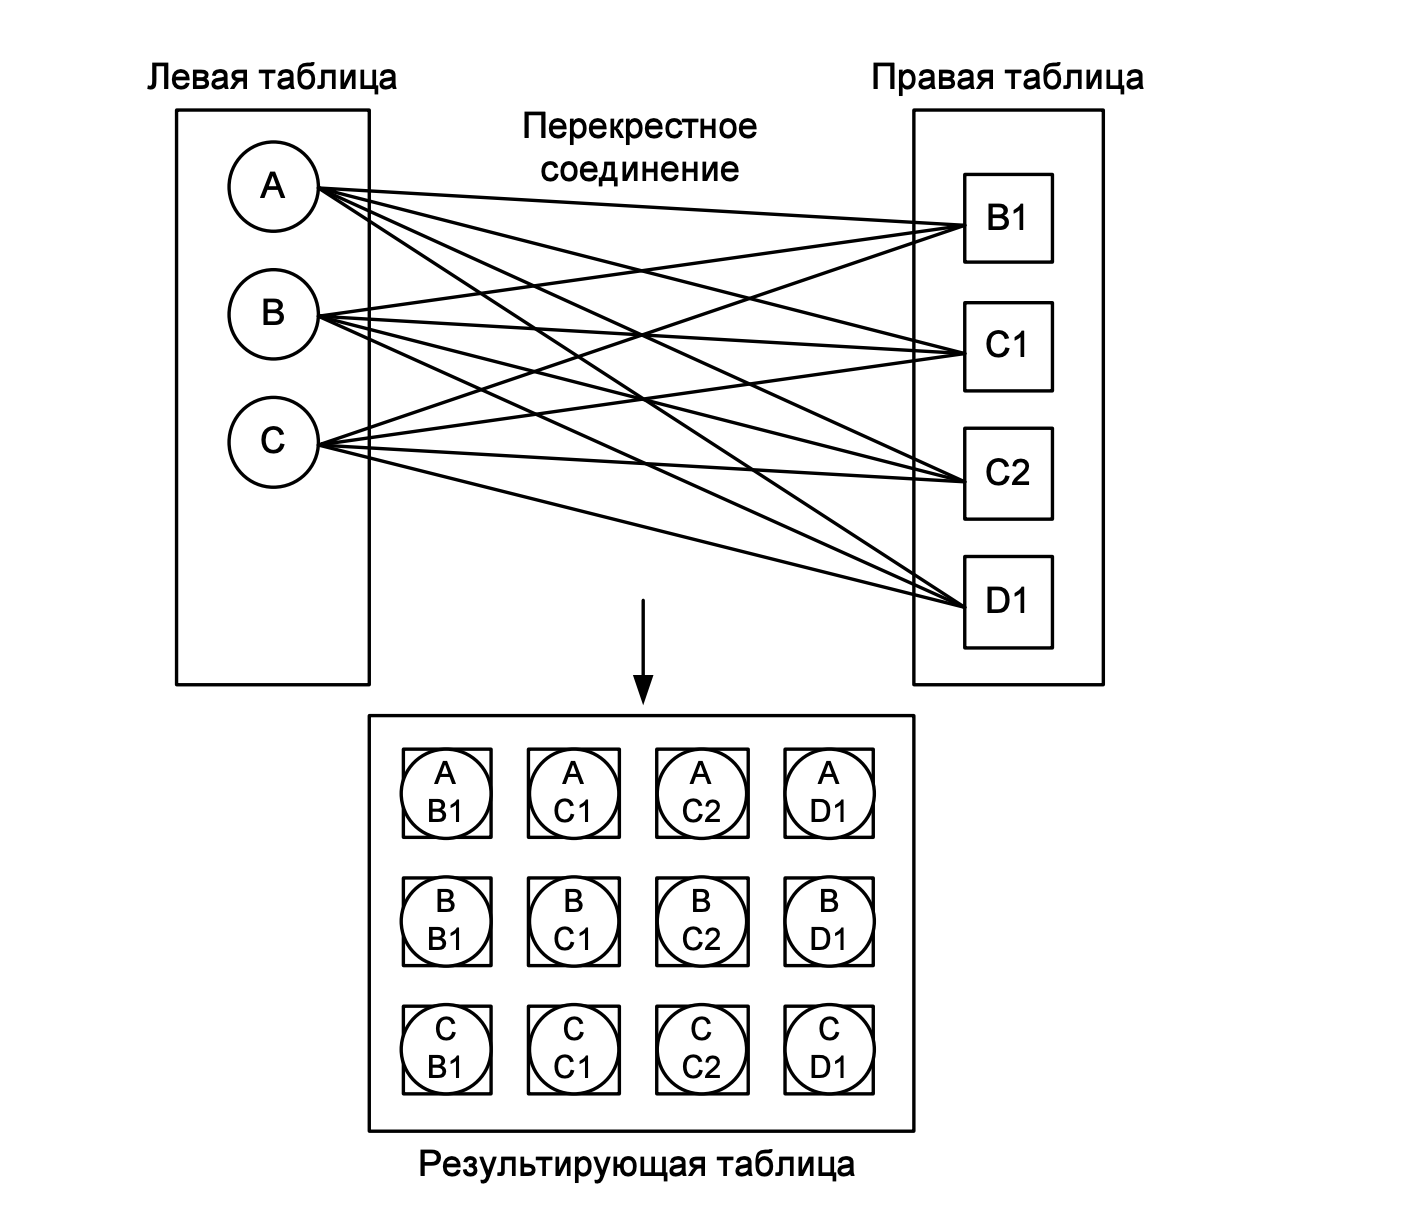
\includegraphics[width=0.8\textwidth]{img/cross.png}
	\end{center}
	\caption{Перекрестное объединение таблиц}
	\captionsetup{justification=centering}
\end{figure}


\subsection{Внутренние соединения INNER JOIN}
С помощью внутренних соединений можно сопоставлять строки из двух таблиц по предикату, как правило, сравнивая значение первичного ключа в одной таблице с внешним ключом в другой. 

\begin{lstlisting}[label=lst:funcReturn, caption=Пример INNER JOIN, language=sql]
	SELECT S.companyname AS supplier, S.country,
		P.productid, P.productname, P.unitprice
   	FROM Production.Suppliers AS S
		INNER JOIN Production.Products AS P
			ON S.supplierid = P.supplierid
   	WHERE S.country = N'Japan'; 
\end{lstlisting}

\begin{figure}[h!]
	\begin{center}
		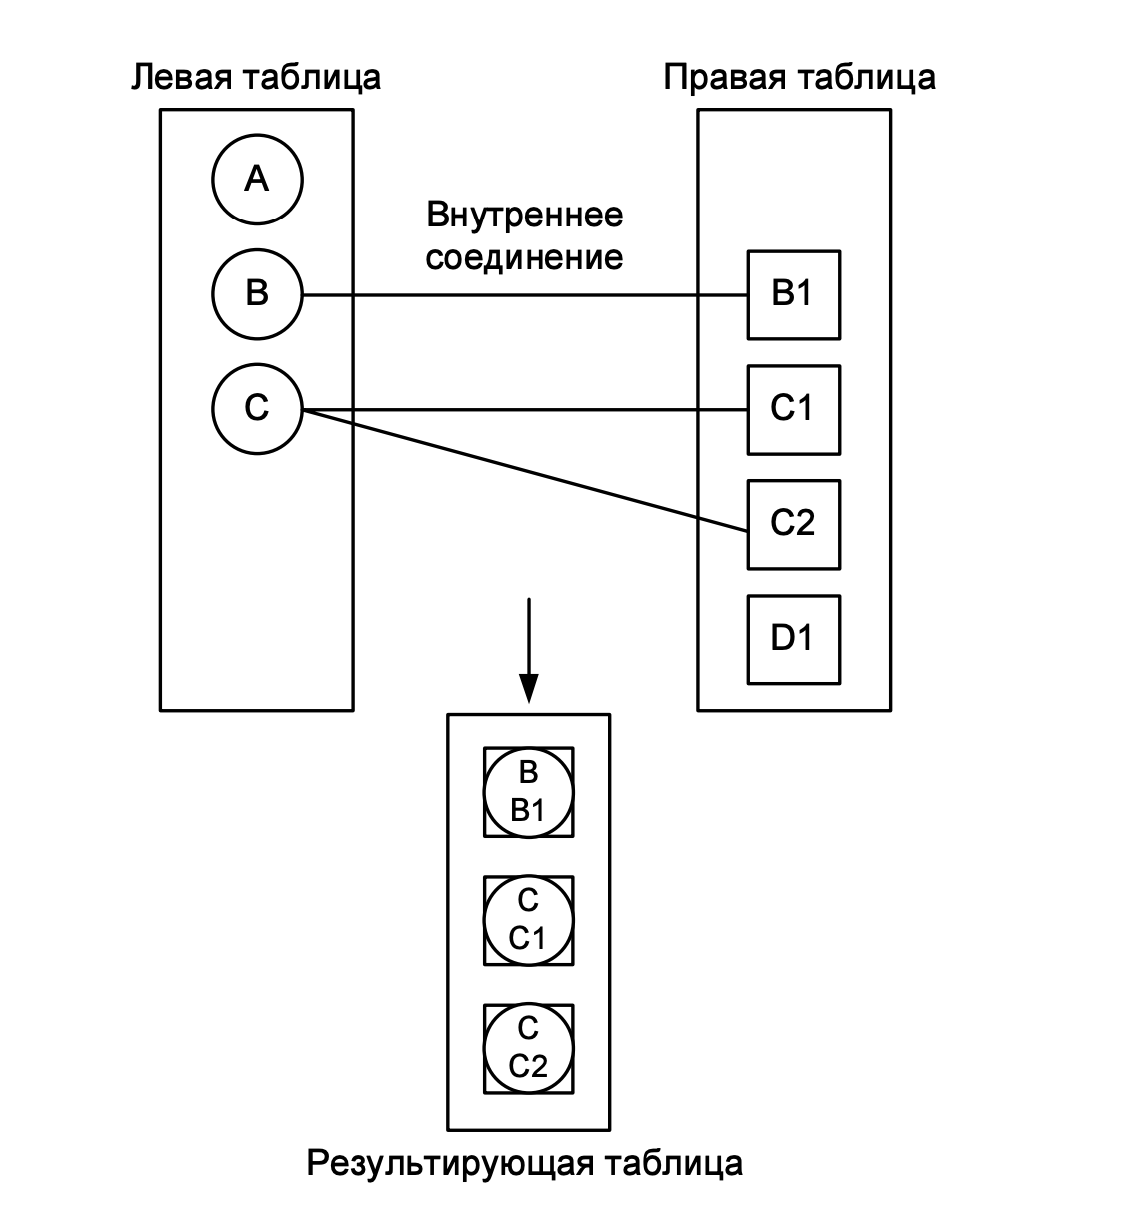
\includegraphics[width=0.8\textwidth]{img/inner.png}
	\end{center}
	\caption{Внутреннее объединение таблиц}
	\captionsetup{justification=centering}
\end{figure}


\begin{figure}[h!]
	\begin{center}
		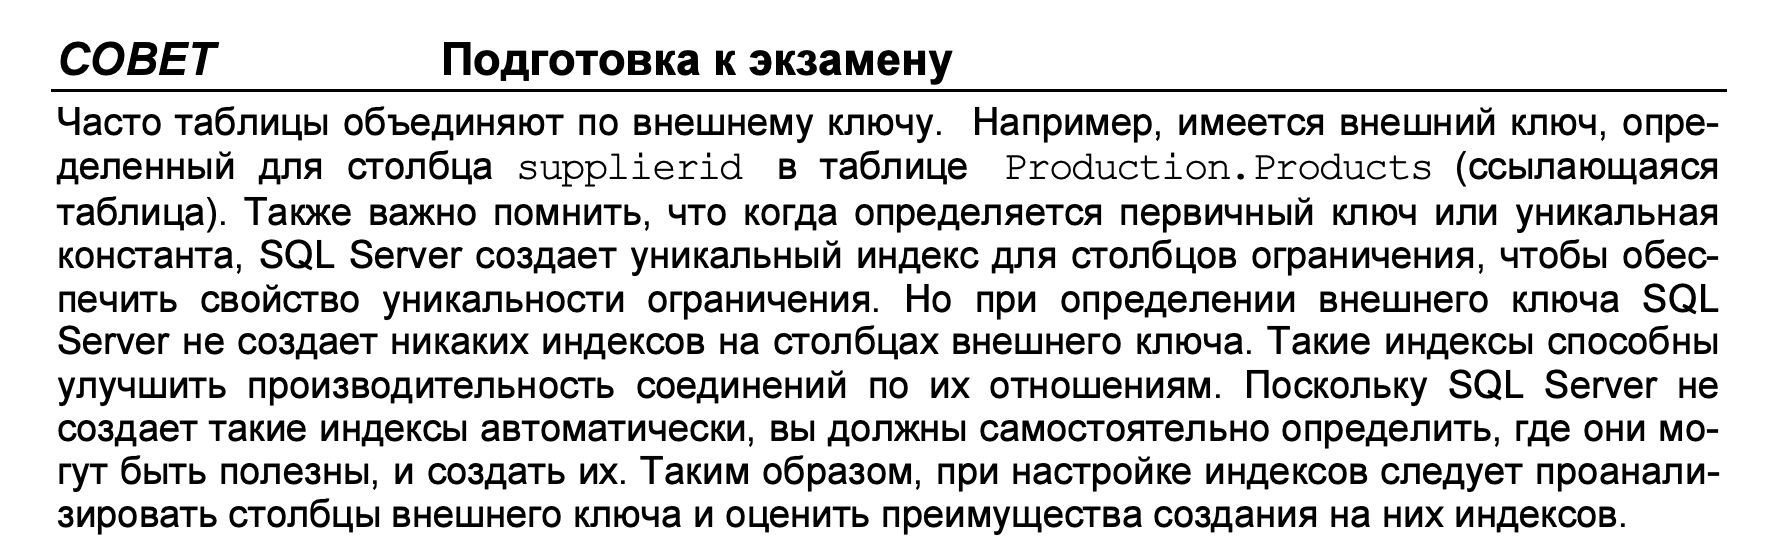
\includegraphics[width=1\textwidth]{img/advice7.png}
	\end{center}
	\captionsetup{justification=centering}
\end{figure}



\subsection{Внешние соединения OUTER JOIN}
С помощью внешнего соединения можно запросить сохранение всех строк из одной или обеих сторон соединения без учета того, имеются ли соответствующие строки в другой стороне. Это осуществляется с помощью предиката ON.

\begin{lstlisting}[label=lst:funcReturn, caption=Пример LEFT JOIN, language=sql]
SELECT S.companyname AS supplier, S.country,
	P.productid, P.productname, P.unitprice
FROM Production.Suppliers AS S
	LEFT OUTER JOIN Production.Products AS P
		ON S.supplierid = P.supplierid
WHERE S.country = N'Japan'; 
\end{lstlisting}

Важно понимать, что в случае внешнего соединения предложения ON и WHERE играют разные роли и поэтому не являются взаимозаменяемыми. Предложение WHERE
по-прежнему играет роль фильтра — а именно, оно сохраняет строки, дающие значение "истина", и отбрасывает строки, дающие значение "ложь" или "неизвестно".
Так, в нашем запросе предложение WHERE фильтрует только поставщиков из Японии, поэтому поставщики из других стран просто не попадают в выходной набор.
Однако предложение ON не является просто фильтром, напротив, его основная задача — сопоставление данных. Иными словами, строка из сохраненной стороны будет возвращена независимо от того, найдет предикат ON совпадение или нет.
\newpage

\begin{figure}[h!]
	\begin{center}
		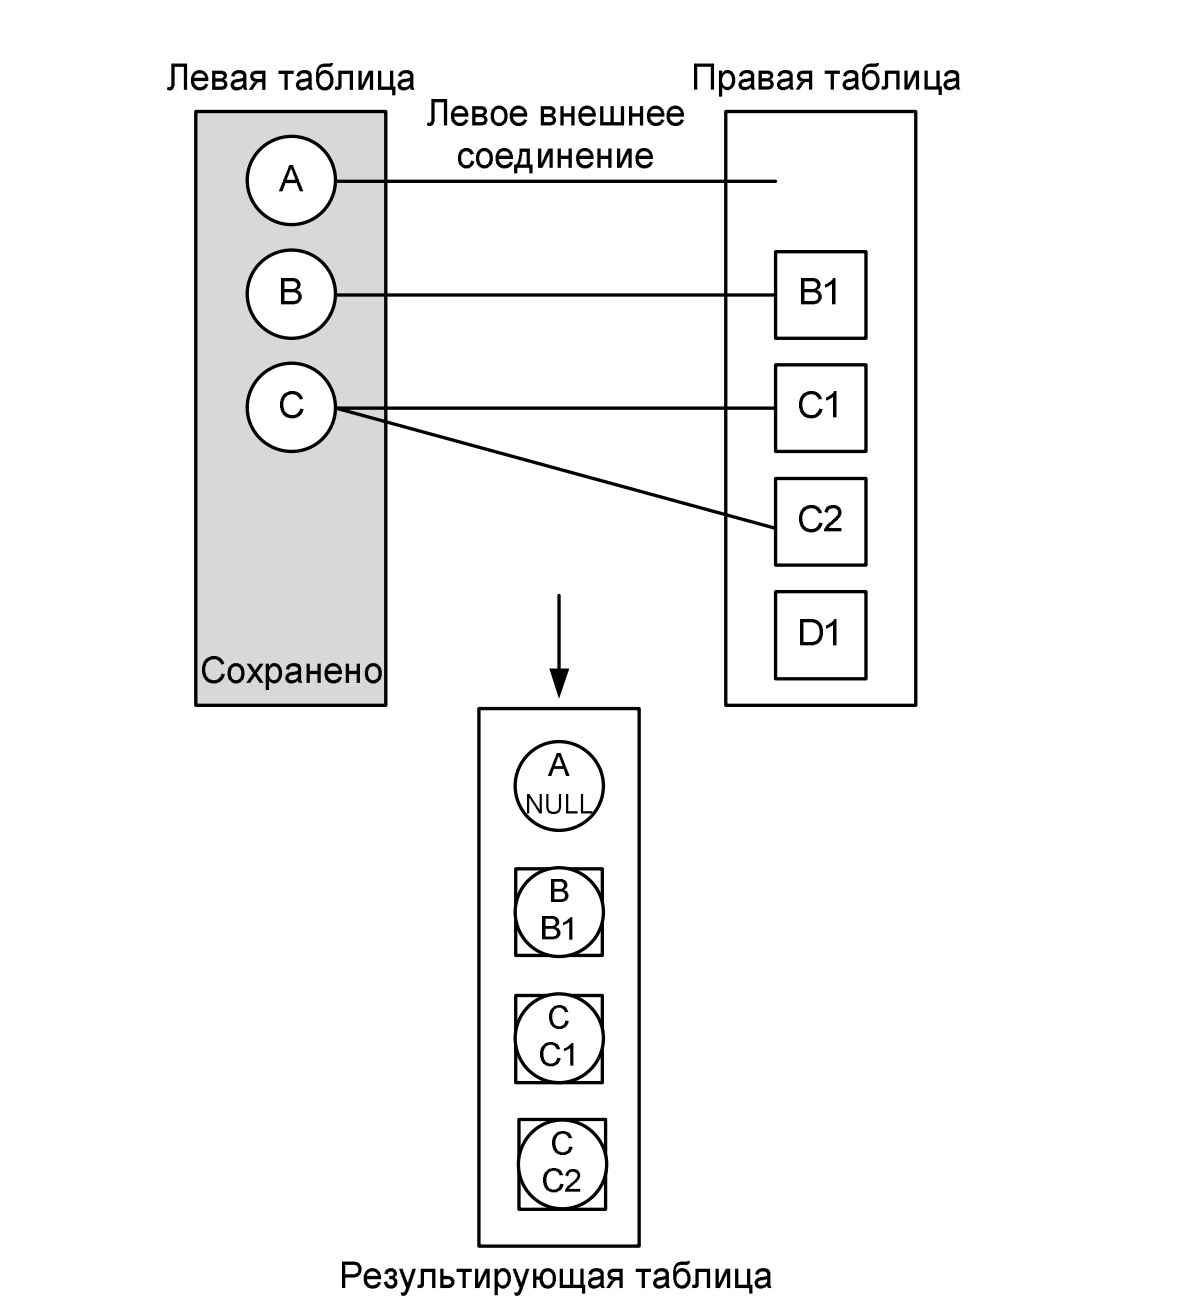
\includegraphics[width=0.5\textwidth]{img/left.png}
	\end{center}
	\captionsetup{justification=centering}
	\caption{Левое внешнее соединение}
\end{figure}

\begin{figure}[h!]
	\begin{center}
		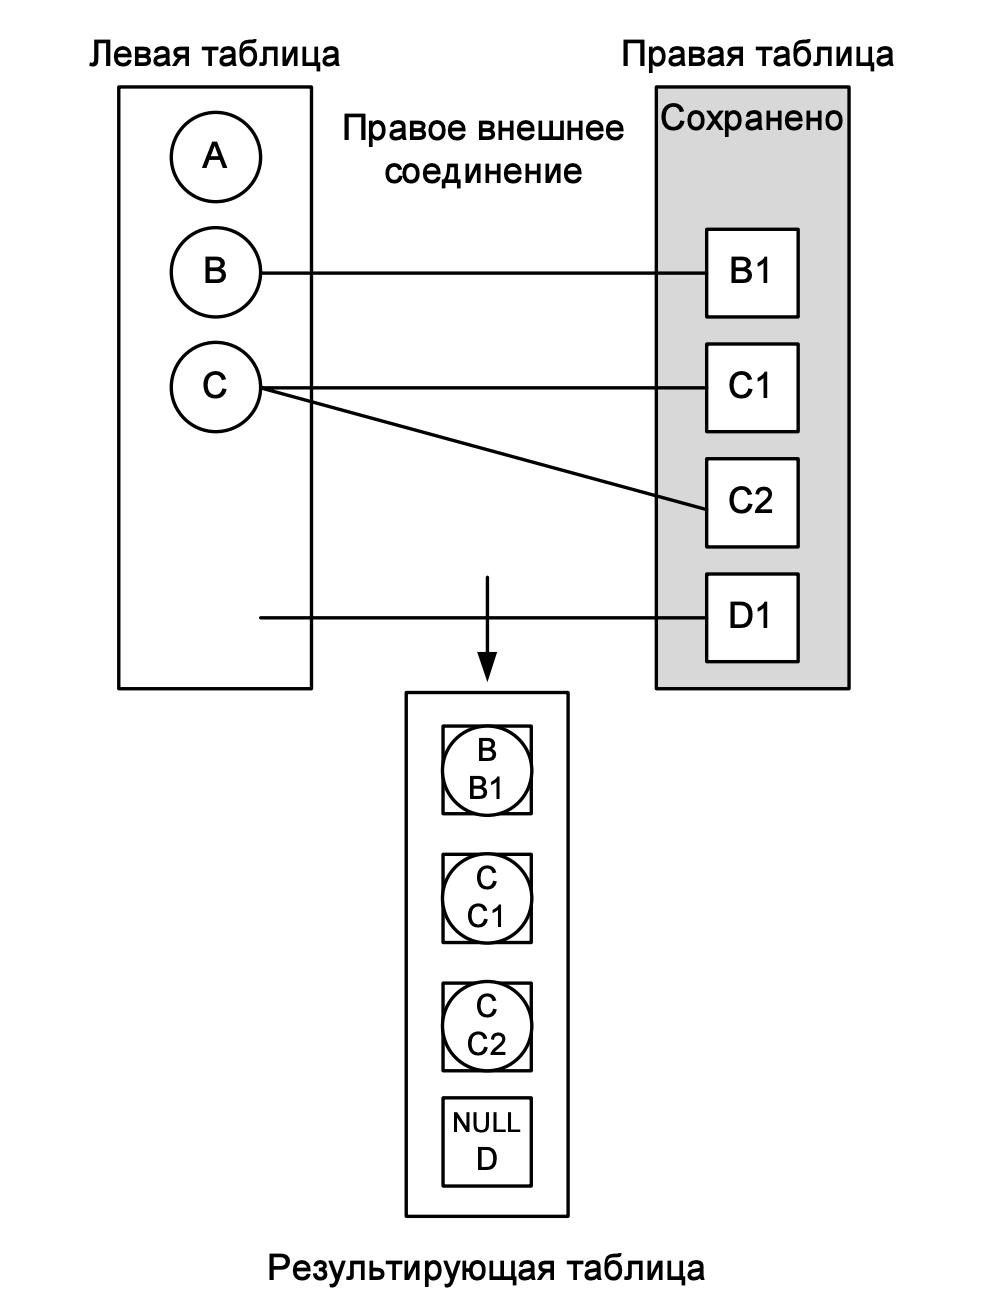
\includegraphics[width=0.5\textwidth]{img/right.png}
	\end{center}
	\caption{Правое внешнее соединение}
	\captionsetup{justification=centering}
\end{figure}

\begin{figure}[h!]
	\begin{center}
		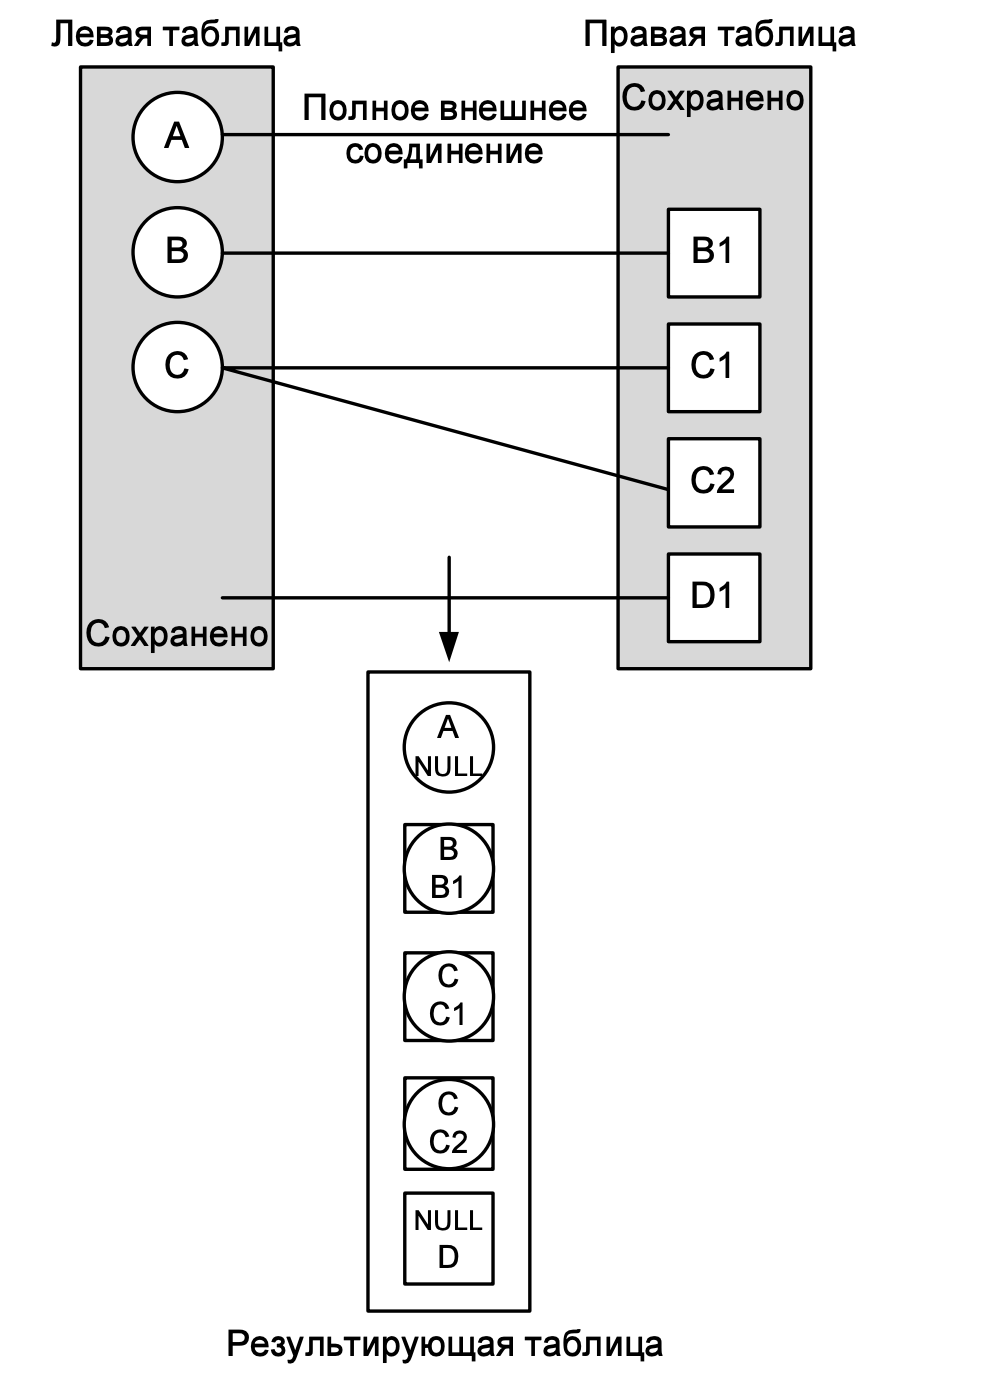
\includegraphics[width=0.5\textwidth]{img/full.png}
	\end{center}
	\captionsetup{justification=centering}
	\caption{Полное внешнее соединение}
\end{figure}


\begin{figure}[h!]
	\begin{center}
		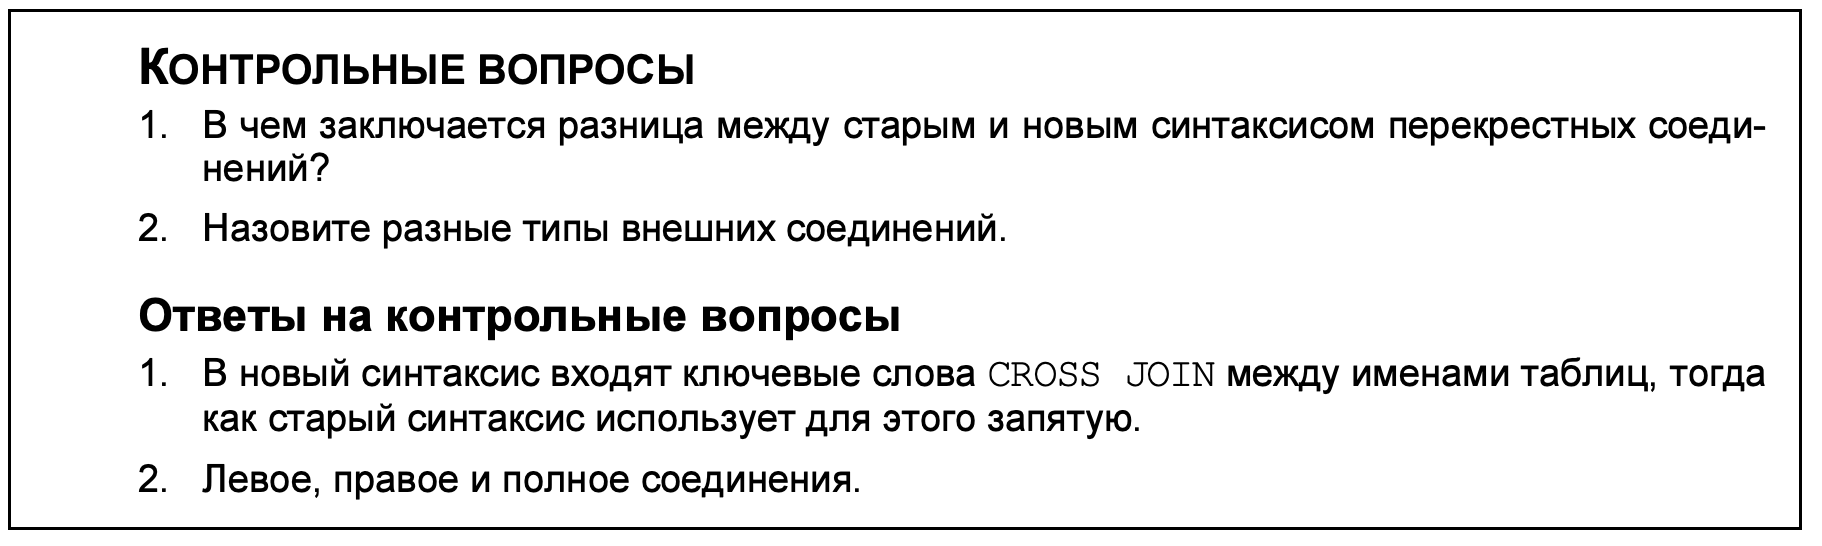
\includegraphics[width=0.9\textwidth]{img/control11.png}
	\end{center}
	\captionsetup{justification=centering}
\end{figure}


\subsection*{Резюме занятия}
\begin{itemize}
	\item Перекрестные соединения возвращают декартово произведение строк обеих сторон. 
	\item Внутренние соединения сопоставляют строки с помощью предиката и возвращают только совпадения.
	\item Внешние соединения сопоставляют строки с помощью предиката и возвращают
	как совпадения, так и несовпадения из таблиц, помеченных как сохраненные.
	\item Запросы с мультисоединениями содержат несколько соединений. В них возможно присутствие разных типов соединений. Логический порядок обработки соединений можно контролировать с помощью круглых скобок или изменением
	положения предложения ON. 
\end{itemize}

\subsection*{Закрепление материала}

\begin{figure}[h!]
	\begin{center}
		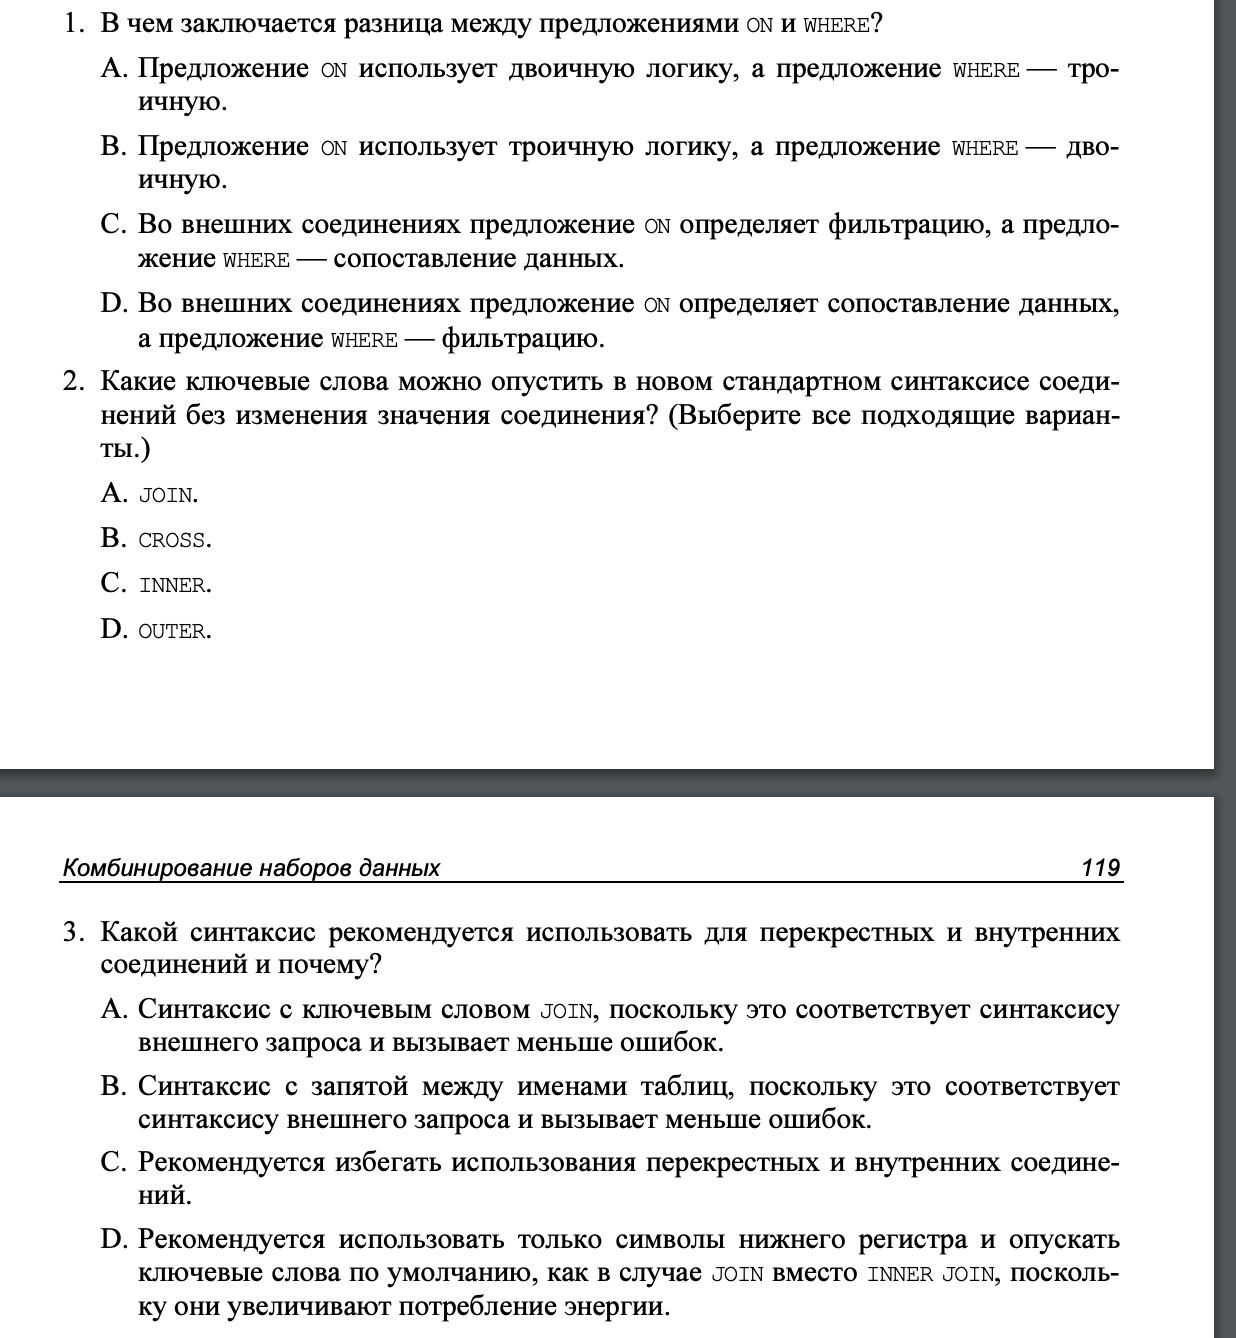
\includegraphics[width=0.7\textwidth]{img/zakrep8.png}
	\end{center}
	\captionsetup{justification=centering}
\end{figure}
\newpage

\subsection*{Ответы}

\begin{figure}[h!]
	\begin{center}
		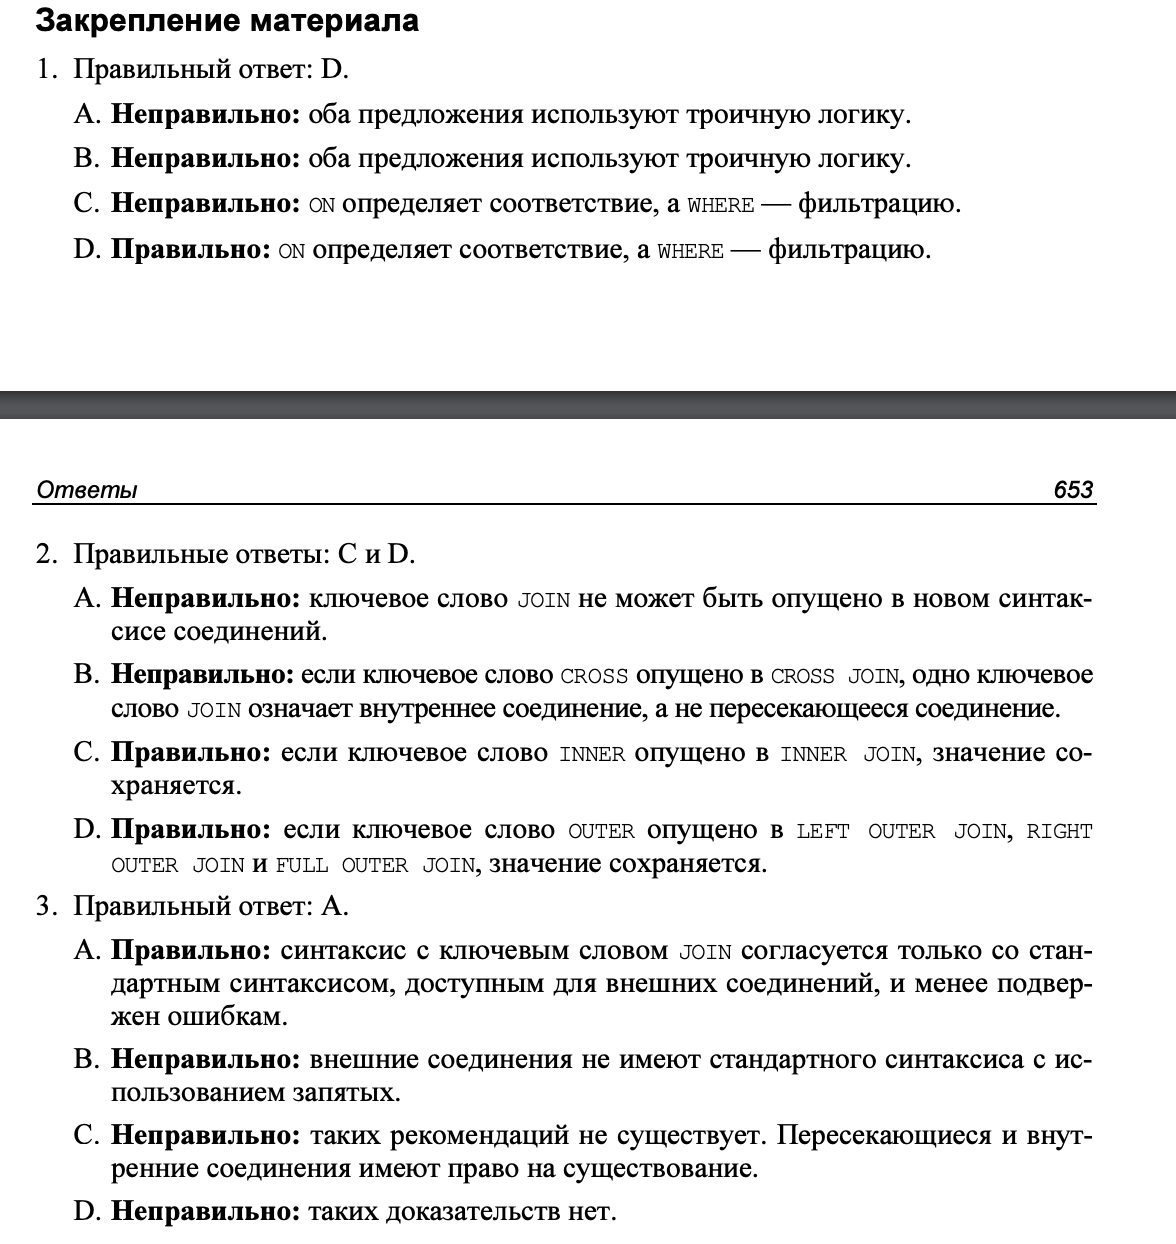
\includegraphics[width=0.9\textwidth]{img/ans8.png}
	\end{center}
	\captionsetup{justification=centering}
\end{figure}
\clearpage


\section{Использование подзапросов, табличных выражений и оператора APPLY}

\subsection{Независимые подзапросы}
Независимые подзапросы — это вложенные запросы, которые не имеют зависимостей от внешнего запроса.


\begin{lstlisting}[label=lst:funcReturn, caption=Пример вложенного подзапроса, language=sql]
SELECT productid, productname, unitprice
FROM Production.Products
WHERE unitprice = (SELECT MIN(unitprice)
						FROM Production.Products); 
\end{lstlisting}


\begin{lstlisting}[label=lst:funcReturn, caption=Пример вложенного запроса с IN, language=sql]
SELECT productid, productname, unitprice
FROM Production.Products
WHERE supplierid IN
	(SELECT supplierid
	FROM Production.Suppliers
	WHERE country = N'Japan'); 
\end{lstlisting}


\subsection{Коррелированные (связанные) подзапросы}

Коррелированные (связанные) подзапросы — это подзапросы, в которых
внутренний запрос имеет ссылку на столбец таблицы во внешнем запросе.
Их использование несколько сложнее по сравнению с независимыми подзапросами, поскольку невозможно просто выделить внутреннюю часть и запустить ее
отдельно.

\begin{lstlisting}[label=lst:funcReturn, language=sql]
SELECT categoryid, productid, productname, unitprice
FROM Production.Products AS P1
WHERE unitprice = (SELECT MIN(unitprice)
	FROM Production.Products AS P2
	WHERE P2.categoryid = P1.categoryid);
	\end{lstlisting}

\begin{lstlisting}[label=lst:funcReturn, language=sql]
SELECT custid, companyname
FROM Sales.Customers AS C
WHERE EXISTS
(SELECT *
	FROM Sales.Orders AS O
	WHERE O.custid = C.custid
	AND O.orderdate = '20070212'); 
\end{lstlisting}
	
Предикат EXISTS принимает подзапрос на вход и возвращает значение <<истина>>,
когда подзапрос возвращает хотя бы одну строку, в противном случае — <<ложь>>. 


\section{Табличные выражения}
Табличные выражения — это именованные запросы. Вы пишете внутренний запрос, который возвращает реляционный результирующий набор, даете ему имя и вызываете его из внешнего запроса. Язык T-SQL поддерживает четыре формы табличных выражений: 

\begin{itemize}
	\item производные таблицы; 
	\item обобщенные табличные выражения (common table expression, CTE);
	\item представления; 
	\item встроенные табличные функции. 
\end{itemize}


\begin{figure}[h!]
	\begin{center}
		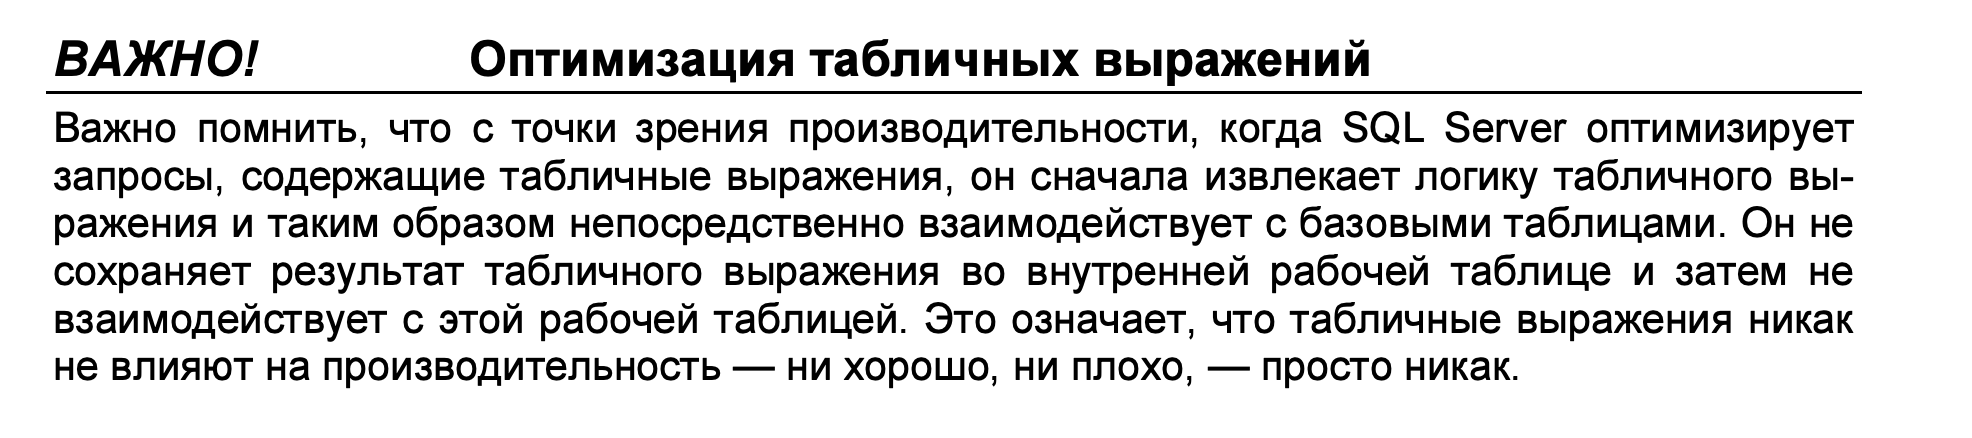
\includegraphics[width=0.9\textwidth]{img/advice8.png}
	\end{center}
	\captionsetup{justification=centering}
\end{figure}

\subsection{Производные таблицы}
Производная таблица — это, возможно, форма табличного выражения, которая более всего похожа на подзапрос, только это подзапрос, возвращающий в качестве
результата целую таблицу.

\begin{lstlisting}[label=lst:funcReturn, language=sql]
	SELECT
		ROW_NUMBER() OVER(PARTITION BY categoryid
			ORDER BY unitprice, productid) AS rownum,
		categoryid, productid, productname, unitprice
   	FROM Production.Products; 
\end{lstlisting}

\begin{figure}[h!]
	\begin{center}
		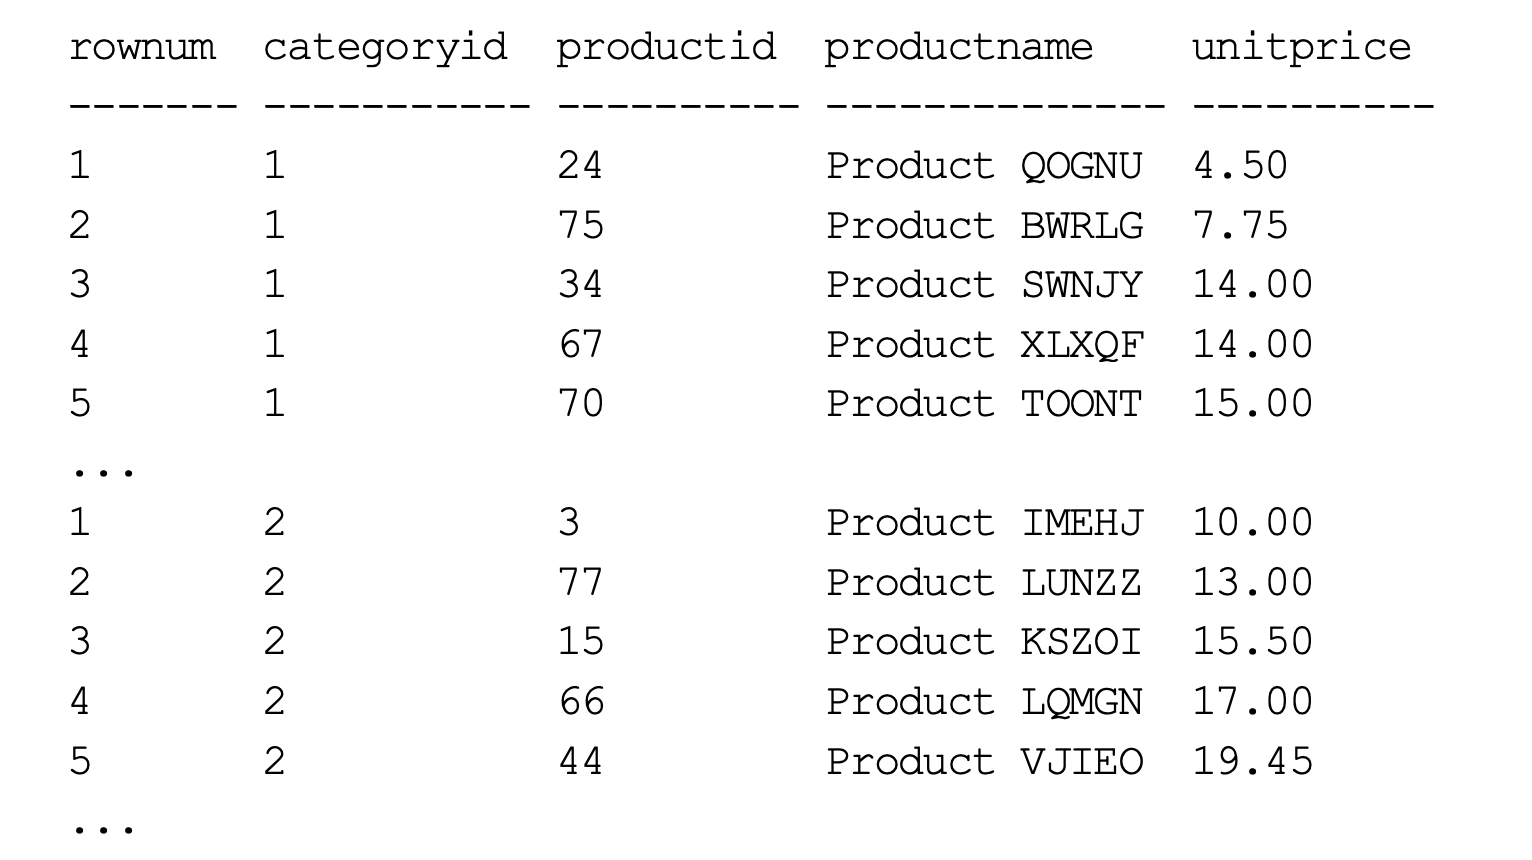
\includegraphics[width=0.6\textwidth]{img/res1.png}
	\end{center}
	\captionsetup{justification=centering}
\end{figure}

Существует пара проблем, связанных с использованием производных таблиц, которые обусловлены тем, что производная таблица определяется в предложении FROM
внешнего запроса. Первая проблема возникает, когда нужно ссылаться на одну
производную таблицу из другой. В таком случае приходится прибегать к вложенным производным таблицам, а вложенность часто усложняет логику, затрудняя
следование ей и увеличивая возможность появления ошибок.

\begin{lstlisting}[label=lst:funcReturn, language=sql]
	SELECT ...
	FROM (SELECT
	 FROM (SELECT ...
	 FROM T1
	 WHERE ...) AS D1
	 WHERE ...) AS D2
	WHERE ...;  
\end{lstlisting}

Другая проблема производных таблиц имеет отношение к свойству "одновременности" языка. Напомним, что все выражения, появляющиеся в одной и той же фазе
логической обработки запроса, концептуально оцениваются в один и тот же момент
времени. Это справедливо и для табличных выражений. В результате имя, присвоенное производной таблице, не видно другим элементам, которые появляются в той
же самой фазе логической обработки запроса, в которой было определено имя производной таблицы. Это означает, что если вы хотите объединить несколько экземпляров одной производной таблицы, вы не сможете это сделать.

\begin{lstlisting}[label=lst:funcReturn, language=sql]
	SELECT ...
	FROM (SELECT ...
	 FROM T1) AS D1
	 INNER JOIN
	 (SELECT ...
	 FROM T1) AS D2
	 ON ...; 
\end{lstlisting}


\subsection{Обобщенные табличные выражения}

Обобщенное табличное выражение (common table expression, CTE) подобно
производной таблице в том смысле, что это именованное табличное выражение, видимое только инструкции, которая его определяет. Так же как запрос
к производной таблице, запрос к CTE включает три основных части:

\begin{itemize}
	\item внутренний запрос; 
	\item имя, которое присваивается запросу и его столбцам;
	\item внешний запрос.
\end{itemize}

\begin{lstlisting}[label=lst:funcReturn, language=sql]
WITH <CTE_name>
AS ( <inner_query> )
<outer_query>; 
\end{lstlisting}

\begin{lstlisting}[label=lst:funcReturn, language=sql]
WITH C AS
(SELECT
	ROW_NUMBER() OVER(PARTITION BY categoryid
	ORDER BY unitprice, productid) AS rownum,
	categoryid, productid, productname, unitprice
	FROM Production.Products)
SELECT categoryid, productid, productname, unitprice
FROM C
WHERE rownum <= 2;
\end{lstlisting}


Такая структура позволяет составлять более чистый код, который проще понимать.
Вам не нужно создавать вложенные CTE, как в случае с производными таблицами.
Если необходимо определить несколько CTE, просто разделите их запятыми.

Отказ от вложенных CTE упрощает следование логике запроса и таким образом снижает возможность появления ошибок. Например,
если нужно сослаться на один CTE из другого, можно использовать следующую
общую форму: 

\begin{lstlisting}[label=lst:funcReturn, language=sql]
	WITH C1 AS
	( SELECT ...
	 FROM T1
	 WHERE ... ),
	C2 AS
	( SELECT
	 FROM C1
	 WHERE ... )
	SELECT ...
	FROM C2
	WHERE ...; 
\end{lstlisting}

Поскольку имя CTE назначено до начала внешнего запроса, можно сослаться на
несколько экземпляров того же самого имени CTE, что невозможно в случае производных таблиц. Общая форма запроса выглядит следующим образом: 

\begin{lstlisting}[label=lst:funcReturn, language=sql]
	WITH C AS
	( SELECT ...
	 FROM T1 )
	SELECT ...
	FROM C AS C1
	INNER JOIN C AS C2
	ON ...; 
\end{lstlisting}

CTE также имеют рекурсивную форму. Тело рекурсивного запроса содержит два
или более запросов, обычно разделенных оператором UNION ALL. По крайней мере,
один запрос в теле CTE, известный как закрепленный элемент, — это запрос, который возвращает реляционный результат. Закрепленный запрос вызывается только
один раз. Кроме того, хотя бы один запрос в теле CTE, называемый рекурсивным
элементом, имеет ссылку на имя CTE. Этот запрос вызывается неоднократно, до
тех пор, пока он не возвратит пустой результирующий набор.

\begin{lstlisting}[label=lst:funcReturn, language=sql]
	WITH EmpsCTE AS
	( SELECT empid, mgrid, firstname, lastname, 0 AS distance
	 FROM HR.Employees
	 WHERE empid = 9 
	 UNION ALL
	 SELECT M.empid, M.mgrid, M.firstname, M.lastname,
	 S.distance + 1 AS distance
	 FROM EmpsCTE AS S
	 JOIN HR.Employees AS M
	 ON S.mgrid = M.empid )
	SELECT empid, mgrid, firstname, lastname, distance
	FROM EmpsCTE;
\end{lstlisting}

\subsection{Представления и встроенные табличные функции}
Чтобы иметь возможность повторного использования, необходимо сохранить определение табличного выражения как объект в базе данных, а для этого можно использовать либо представления, либо встроенные функции, возвращающие табличное значение (табличные функции).
Главное различие между представлениями и встроенными табличными функциями
заключается в том, что первые не принимают входные параметры, а вторые — принимают.

\begin{lstlisting}[label=lst:funcReturn, language=sql]
IF OBJECT_ID('Sales.RankedProducts', 'V') IS NOT NULL
DROP VIEW Sales.RankedProducts;
GO
CREATE VIEW Sales.RankedProducts
AS
SELECT ROW_NUMBER() OVER(PARTITION BY categoryid
 ORDER BY unitprice, productid) AS rownum,
 categoryid, productid, productname, unitprice
FROM Production.Products;
GO 
\end{lstlisting}

Предположим, вы хотите инкапсулировать логику того запроса в табличное выражение для повторного использования,
а также параметризовать входные данные сотрудника вместо использования константы 9. Этого можно достигнуть с помощью встроенной табличной функции со
следующим определением:

\begin{lstlisting}[label=lst:funcReturn, language=sql]
IF OBJECT_ID('HR.GetManagers', 'IF') IS NOT NULL DROP FUNCTION HR.GetManagers;
GO
CREATE FUNCTION HR.GetManagers(@empid AS INT) RETURNS TABLE
AS
RETURN
	WITH EmpsCTE AS
	( SELECT empid, mgrid, firstname, lastname, 0 AS distance
	FROM HR.Employees
	WHERE empid = @empid
	UNION ALL
	SELECT M.empid, M.mgrid, M.firstname, M.lastname,
	S.distance + 1 AS distance
	FROM EmpsCTE AS S
	JOIN HR.Employees AS M
	ON S.mgrid = M.empid )

	SELECT empid, mgrid, firstname, lastname, distance
FROM EmpsCTE;
GO 
\end{lstlisting}


\section{Оператор APPLY}
По сравнению с объединением, оператор APPLY интересен тем,
что правое табличное выражение может быть связано с левой таблицей; другими
словами, внутренний запрос в правом табличном выражении может иметь ссылку
на элемент из левой таблицы.

\subsection{CROSS APPLY}

\begin{figure}[h!]
	\begin{center}
		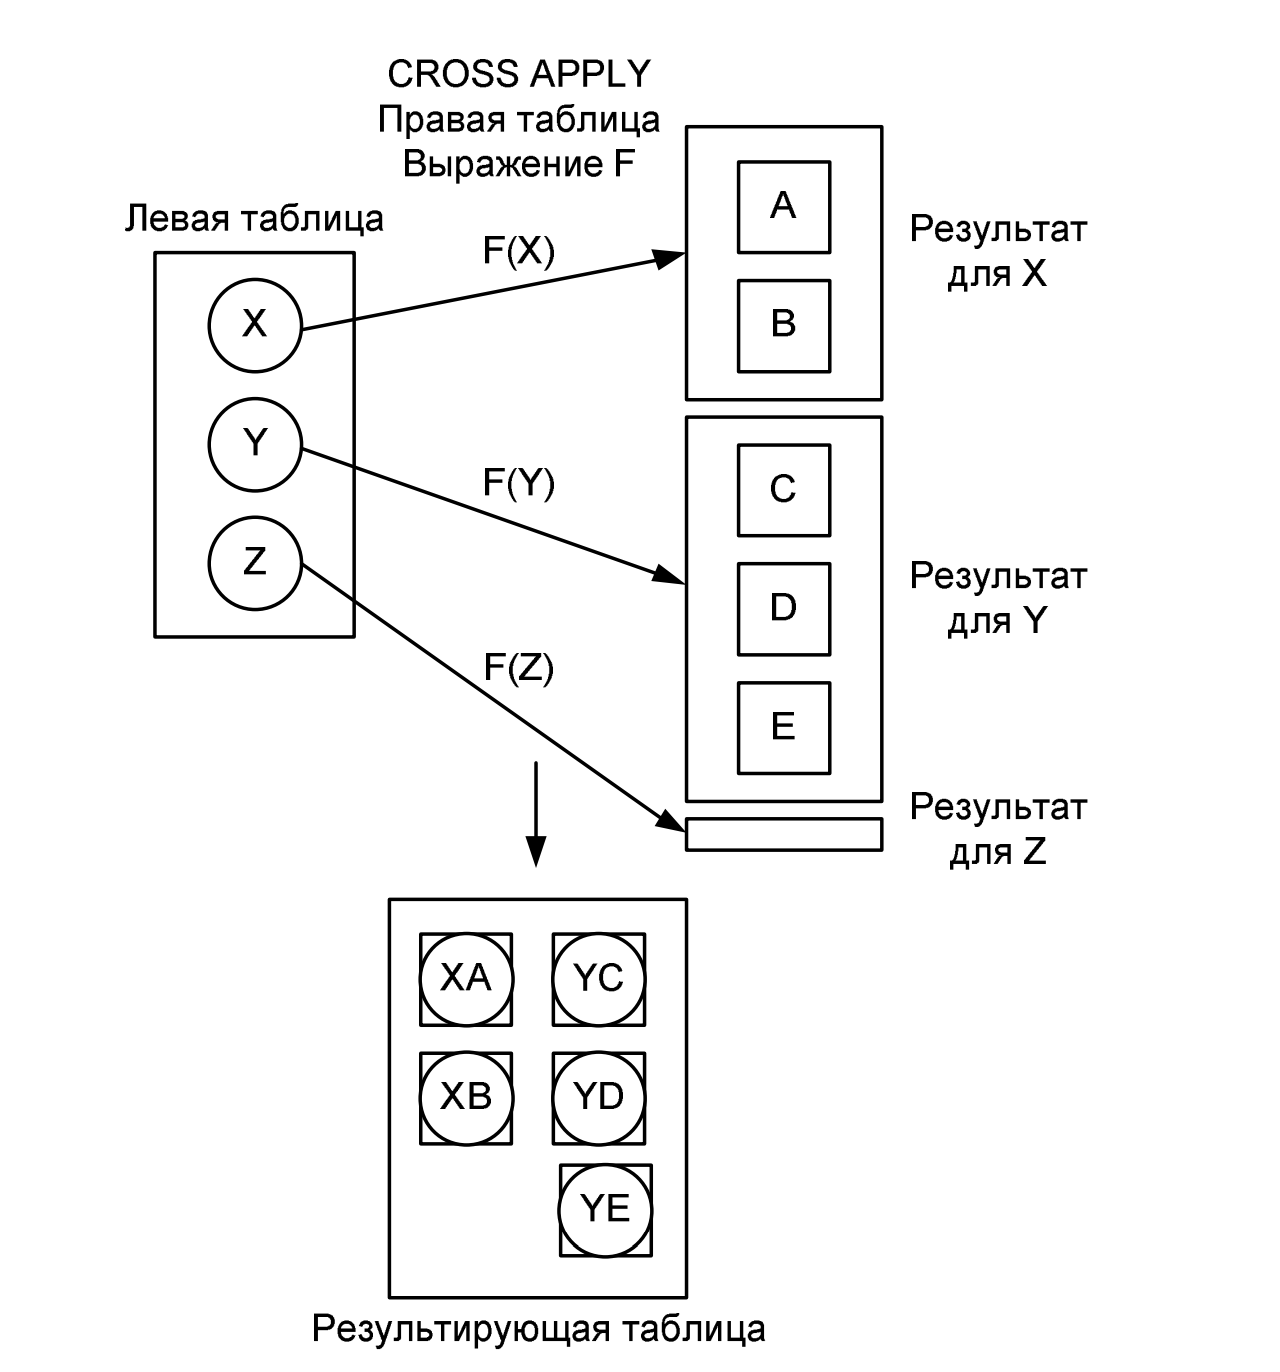
\includegraphics[width=0.9\textwidth]{img/crossapply.png}
	\end{center}
	\captionsetup{justification=centering}
\end{figure}


\subsection{OUTER APPLY}

Оператор OUTER APPLY делает то же самое, что и оператор CROSS APPLY, и кроме этого включает в результат строки с левой стороны, которые возвращают пустой набор
с правой стороны. Значения NULL используются как заменители для результирующих столбцов с правой стороны. Иными словами, оператор OUTER APPLY сохраняет
записи левой стороны.


\begin{figure}[h!]
	\begin{center}
		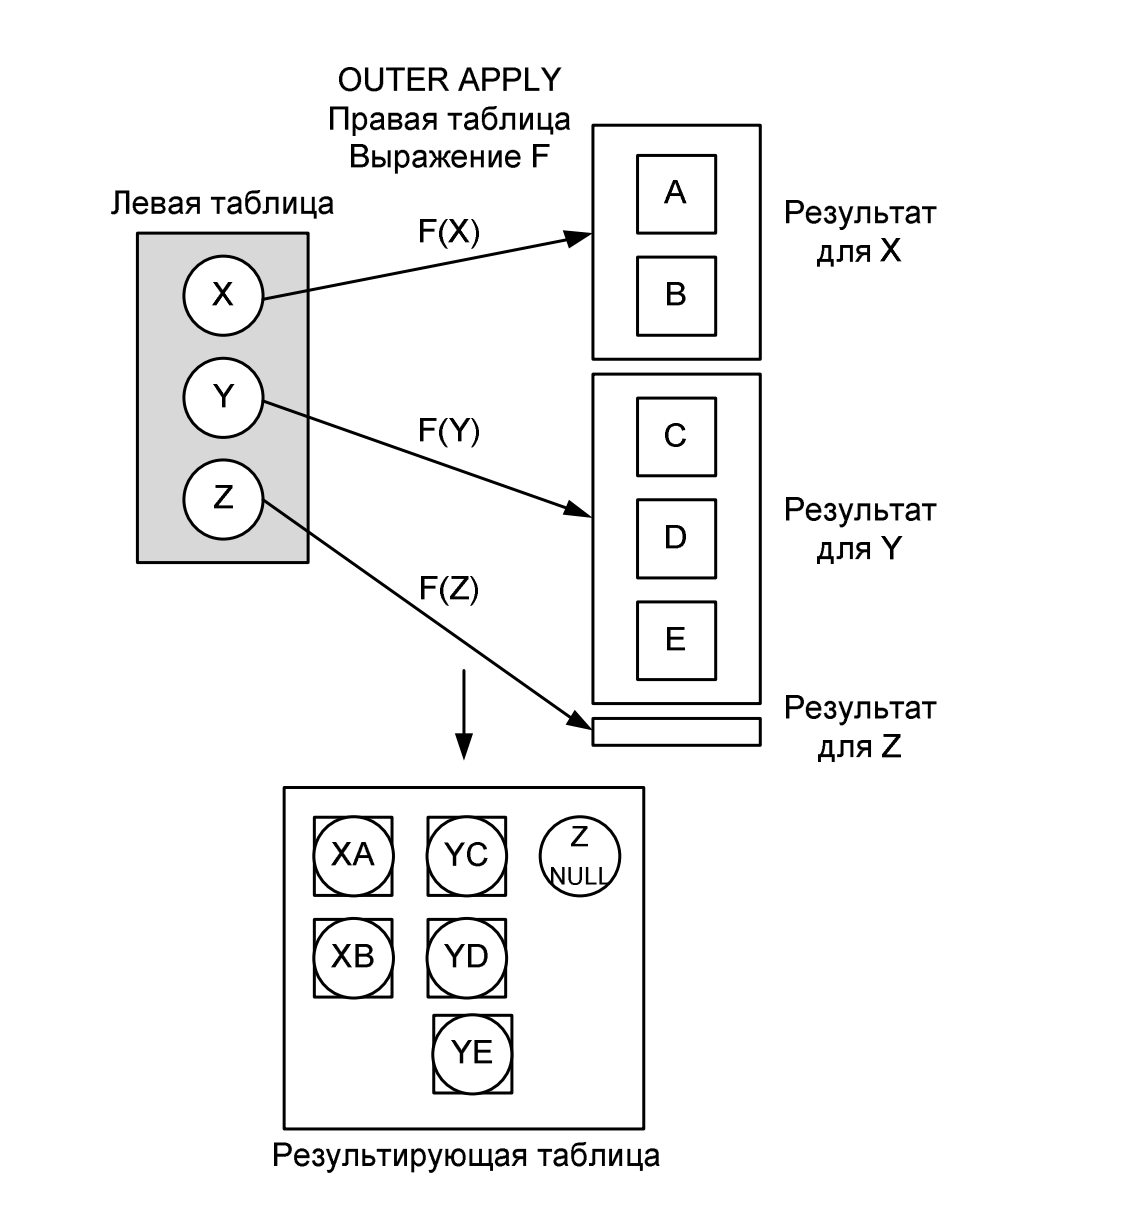
\includegraphics[width=0.9\textwidth]{img/outerapply.png}
	\end{center}
	\captionsetup{justification=centering}
\end{figure}


\begin{figure}[h!]
	\begin{center}
		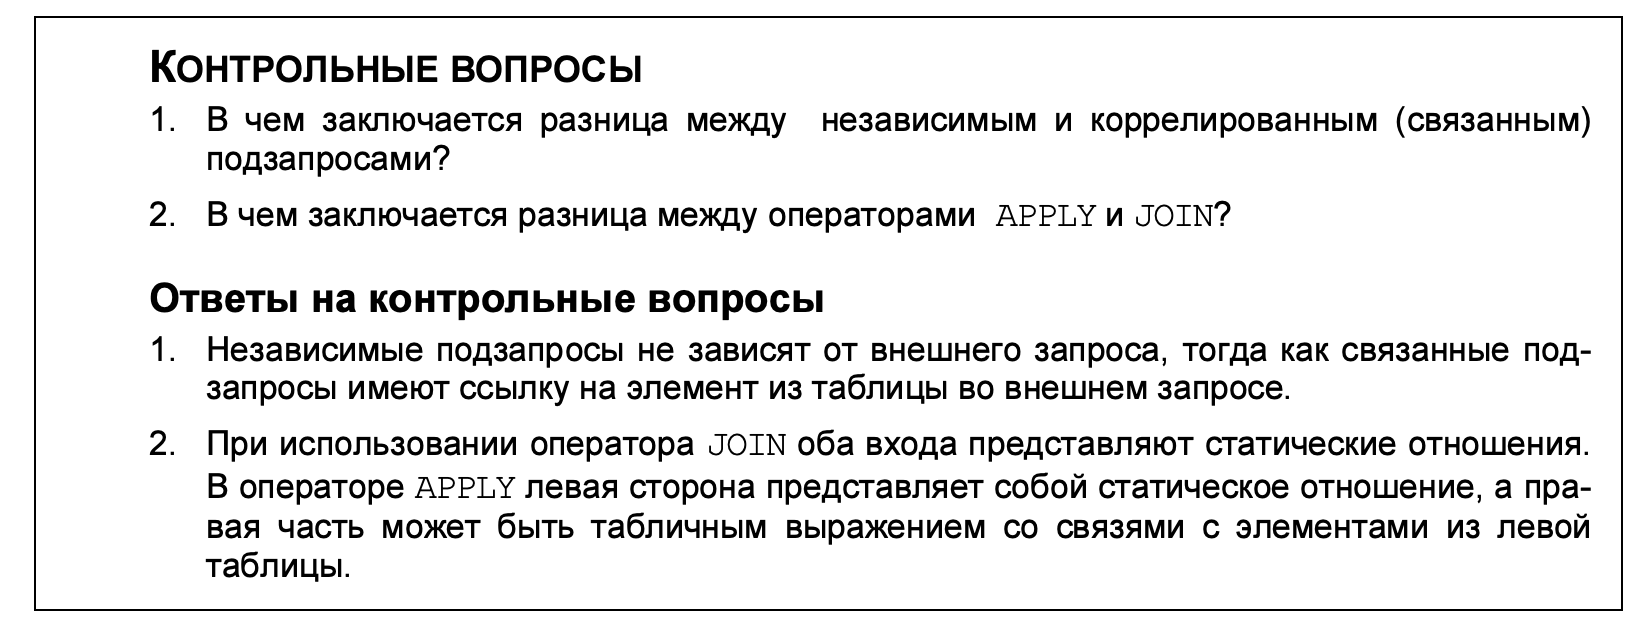
\includegraphics[width=0.9\textwidth]{img/control12.png}
	\end{center}
	\captionsetup{justification=centering}
\end{figure}

\subsection*{Практикум}

\begin{figure}[h!]
	\begin{center}
		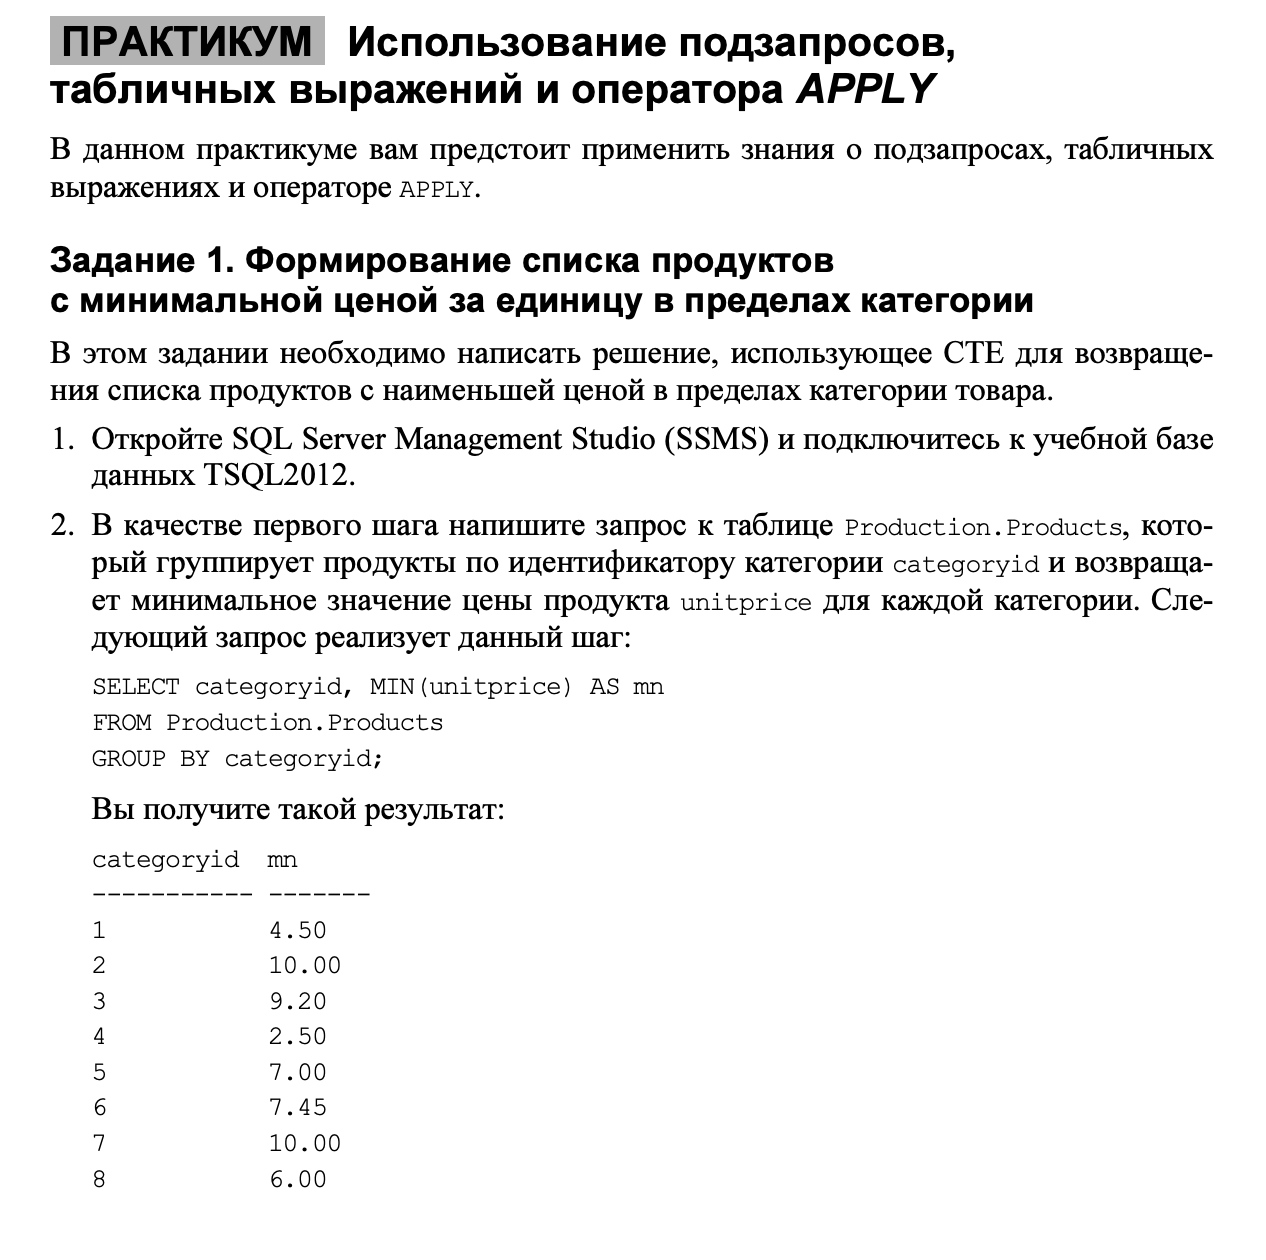
\includegraphics[width=0.9\textwidth]{img/ex7.png}
	\end{center}
	\captionsetup{justification=centering}
\end{figure}


\begin{figure}[h!]
	\begin{center}
		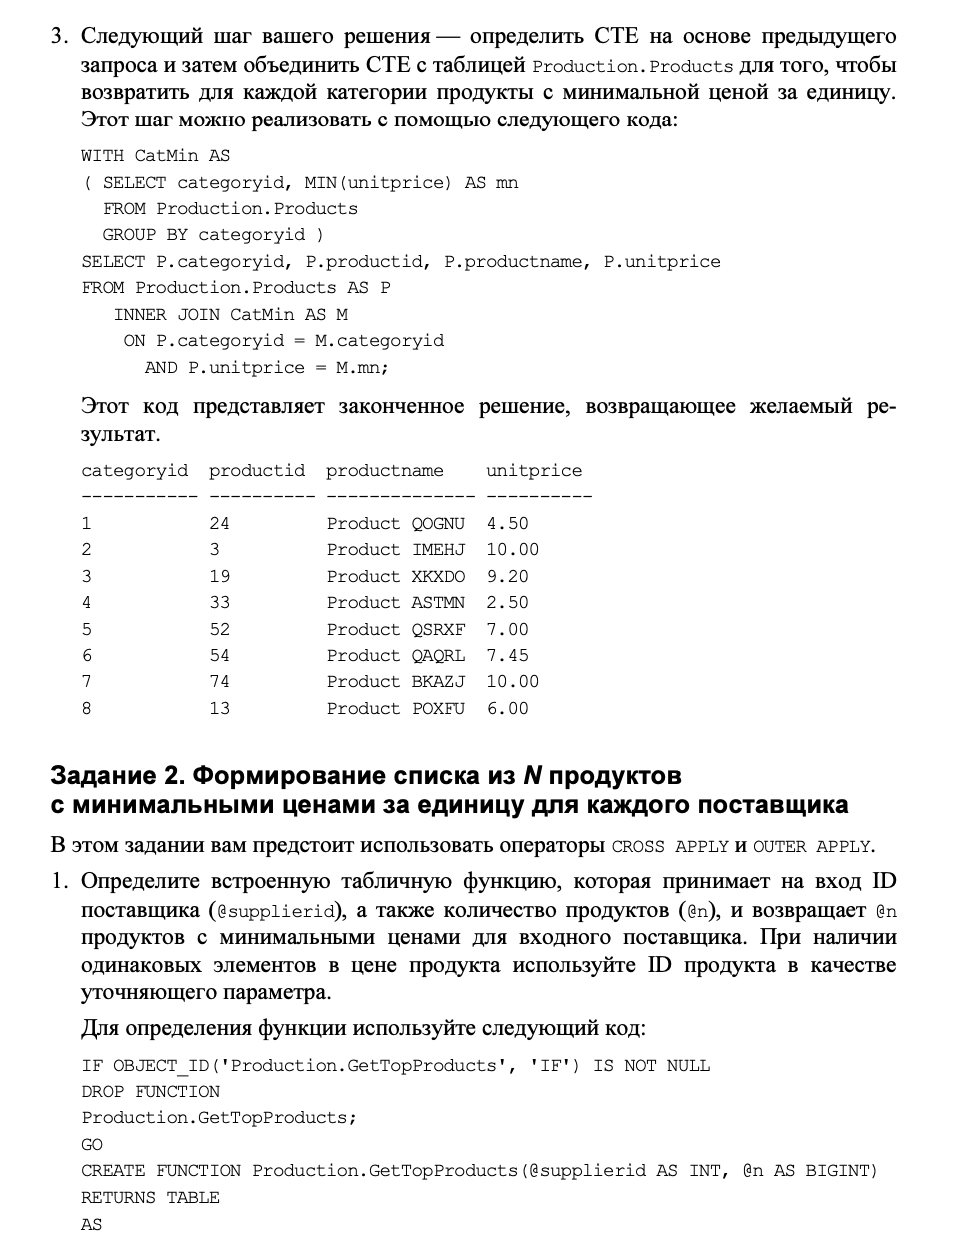
\includegraphics[width=0.9\textwidth]{img/ex8.png}
	\end{center}
	\captionsetup{justification=centering}
\end{figure}
\clearpage


\begin{figure}[h!]
	\begin{center}
		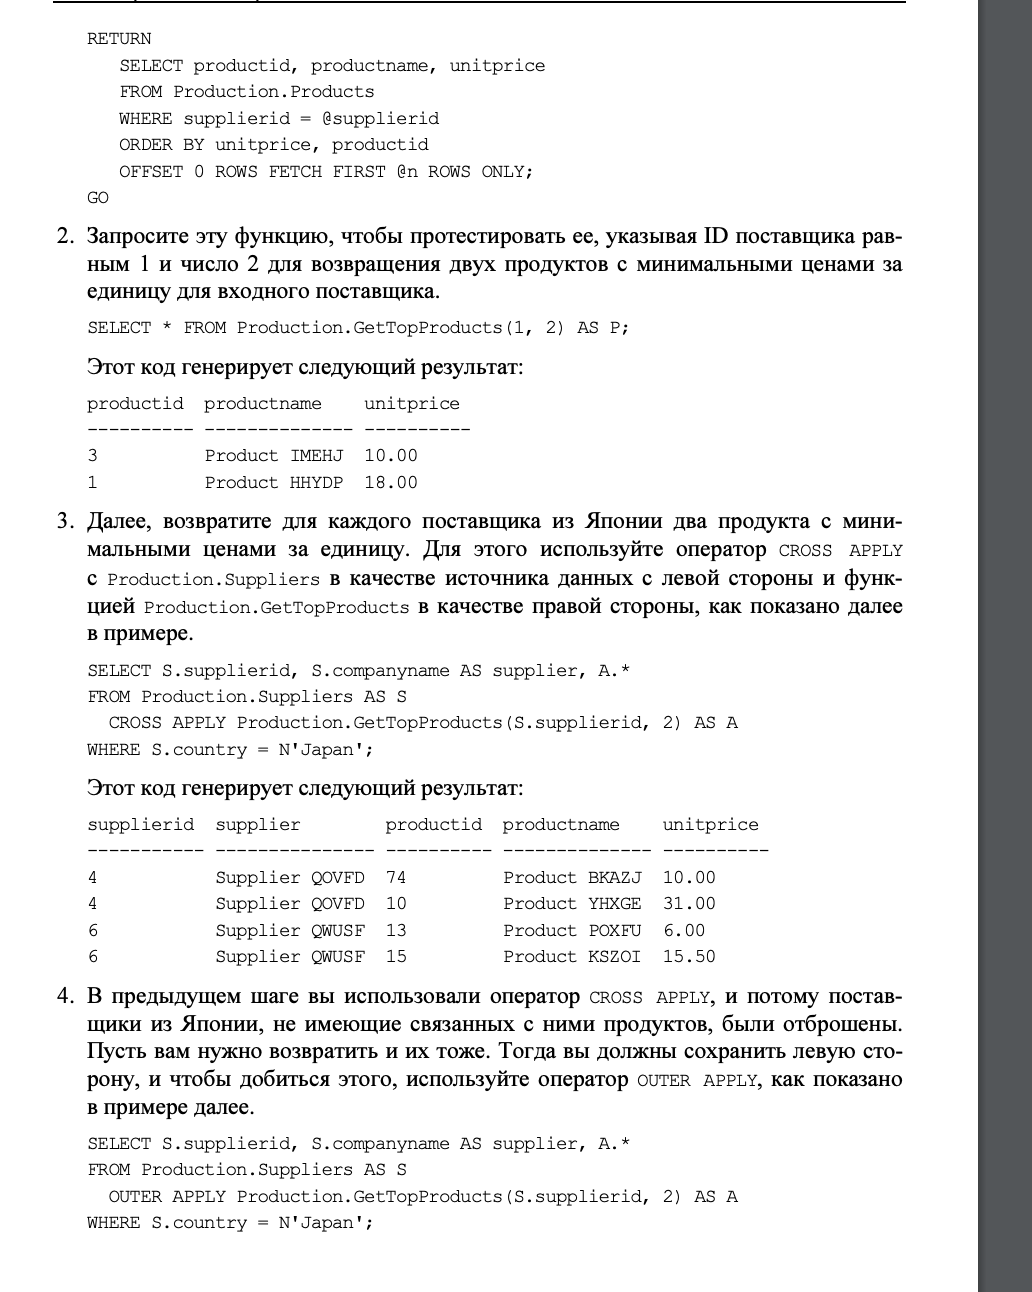
\includegraphics[width=0.7\textwidth]{img/ex9.png}
	\end{center}
	\captionsetup{justification=centering}
\end{figure}

\begin{figure}[h!]
	\begin{center}
		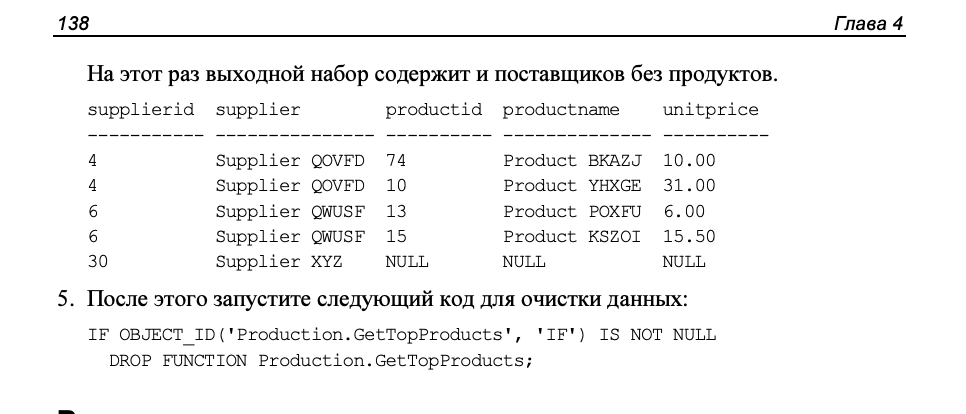
\includegraphics[width=0.7\textwidth]{img/ex10.png}
	\end{center}
	\captionsetup{justification=centering}
\end{figure}


\subsection*{Резюме занятия}
\begin{itemize}
	\item С помощью подзапросов можно вкладывать запросы друг в друга. Можно использовать как независимые, так и связанные подзапросы. Подзапросы могут
	возвращать в качестве результата одно значение, несколько значений или таблицу.
	\item Язык T-SQL поддерживает четыре вида табличных выражений, которые являются именованными выражениями запросов. Производные таблицы и CTE —
	это виды табличных выражений, доступных только для инструкции, в которой
	они определены. Представления и встроенные табличные функции представляют собой повторно используемые табличные выражения, определения которых
	сохраняются в базе данных в виде объектов. Представления не поддерживают
	входные параметры, тогда как встроенные табличные функции поддерживают
	их. 
	\item Оператор APPLY обрабатывает два табличных выражения как входные наборы.
	Он применяет правое табличное выражение к каждой строке из левой стороны.
	Внутренний запрос в правом табличном выражении может иметь связи с элементами из левой таблицы. Оператор APPLY имеет два варианта. Вариант CROSS
	APPLY не возвращает левые строки, которые возвращают пустой набор из правой
	стороны. Оператор OUTER APPLY сохраняет левую сторону и поэтому возвращает
	строки из набора данных с левой стороны, когда правая сторона возвращает
	пустой набор. Значения NULL используются для замещения атрибутов правой
	стороны во внешних строках. 
\end{itemize}


\subsection*{Закрепление материала}

\begin{figure}[h!]
	\begin{center}
		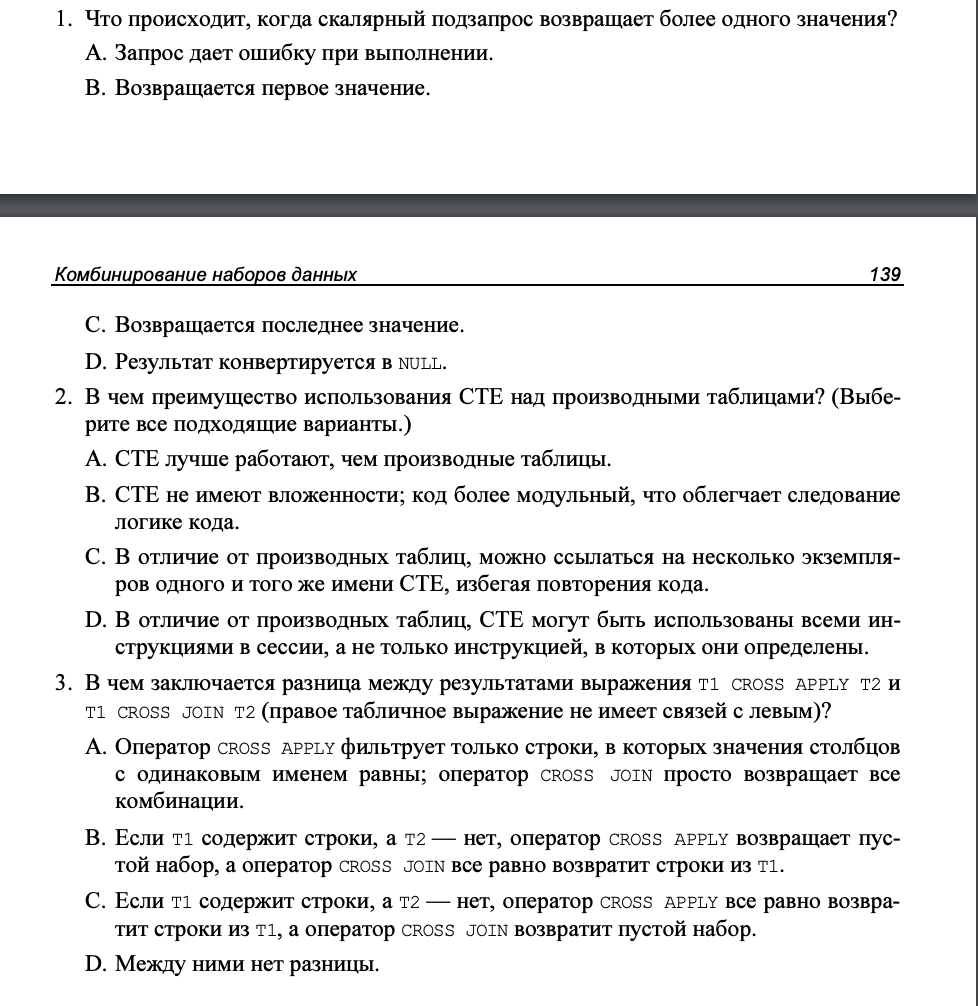
\includegraphics[width=0.9\textwidth]{img/zakrep9.png}
	\end{center}
	\captionsetup{justification=centering}
\end{figure}
\clearpage

\subsection*{Ответы}

\begin{figure}[h!]
	\begin{center}
		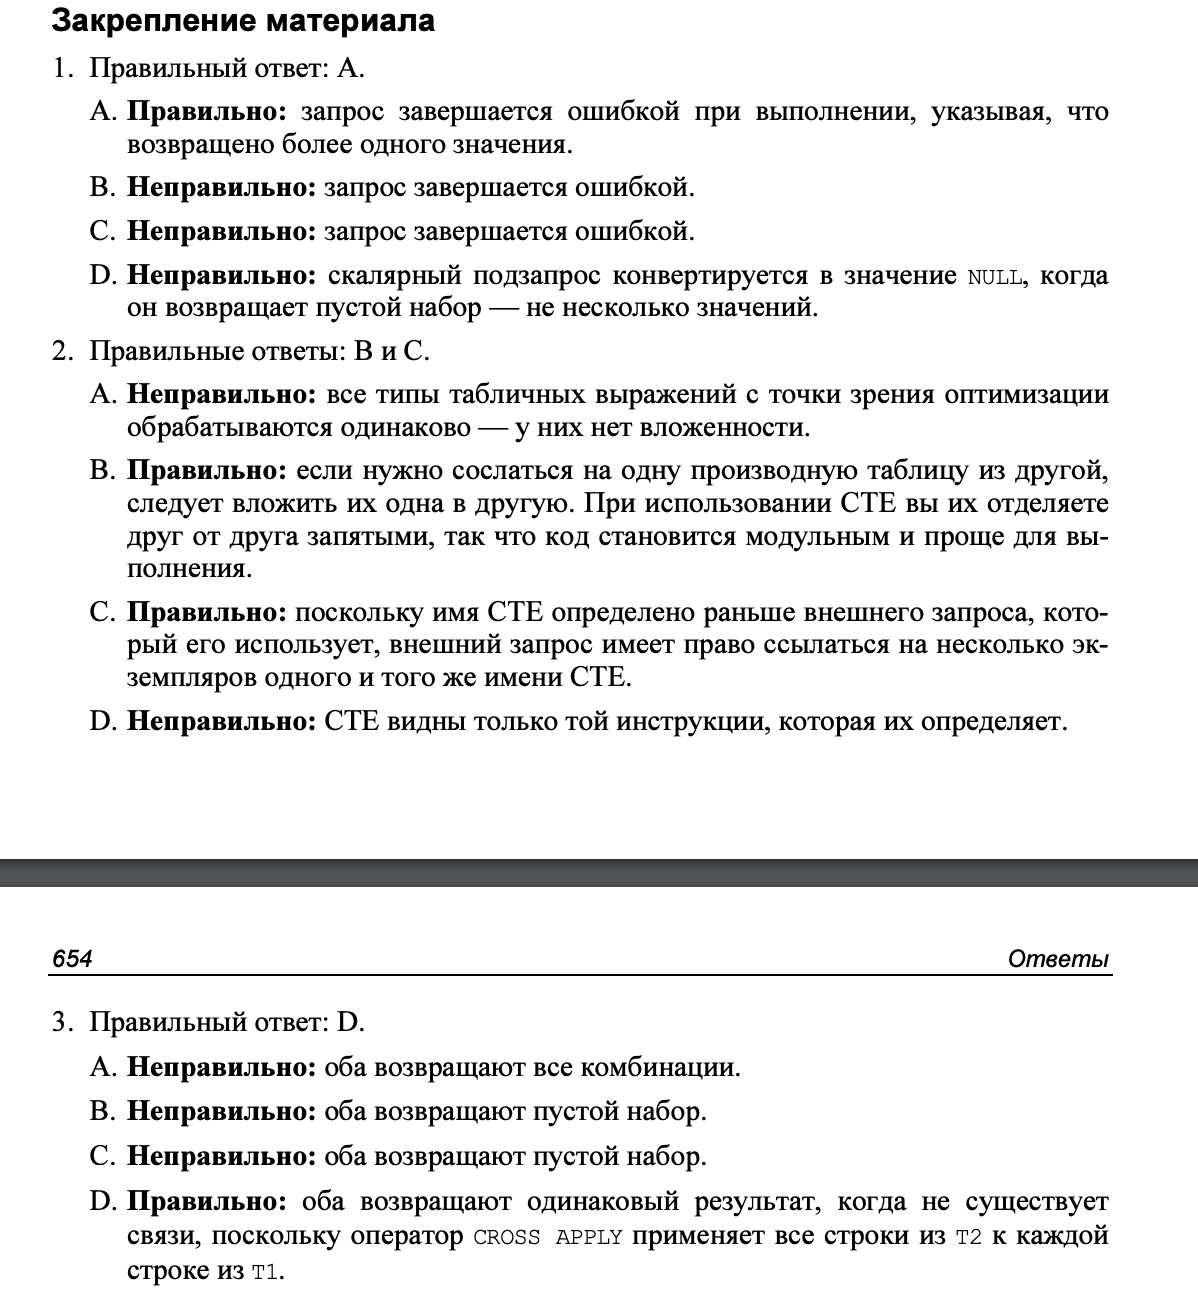
\includegraphics[width=0.9\textwidth]{img/ans9.png}
	\end{center}
	\captionsetup{justification=centering}
\end{figure}



\section{Использование операторов работы с наборами}

Язык T-SQL поддерживает три оператора работы с наборами: UNION, INTERSECT и EXCEPT; также в нем поддерживается оператор UNION ALL
для работы с наборами типа multiset.


\begin{lstlisting}[label=lst:funcReturn, language=sql]
<query 1>
<set operator>
<query 2>
[ORDER BY <order_by_list>] 
\end{lstlisting}

Существует несколько правил, которым необходимо следовать при использовании
операторов работы с наборами:

\begin{itemize}
	\item Поскольку полные строки сопоставляются между результирующими наборами,
	количество столбцов в запросах должно совпадать и типы соответствующих
	столбцов должны быть сравнимыми (неявно конвертируемыми). 
	\item Операторы работы с наборами рассматривают два значения NULL как равные при
	сравнении. Это довольно необычно по сравнению с предложениями фильтрации, такими как WHERE и ON.
	\item Поскольку речь идет об операторах работы с наборами, а не операторах курсора,
	отдельные запросы не могут иметь предложений ORDER BY. 
	\item При желании можно добавить предложение ORDER BY, которое определяет порядок сортировки результата, возвращаемого оператором работы с наборами. 
	\item Имена столбцов для результирующих столбцов определяются первым запросом. 
\end{itemize}
	
\subsection{Операторы UNION и UNION ALL}

Оператор работы с наборами UNION объединяет результаты двух входных запросов.
В качестве примера использования оператора UNION рассмотрим следующий запрос,
который возвращает местоположения сотрудников, клиентов или и тех, и других. 

\begin{lstlisting}[label=lst:funcReturn, language=sql]
SELECT country, region, city
FROM HR.Employees
UNION
SELECT country, region, city
FROM Sales.Customers; 
\end{lstlisting}


\begin{figure}[h!]
	\begin{center}
		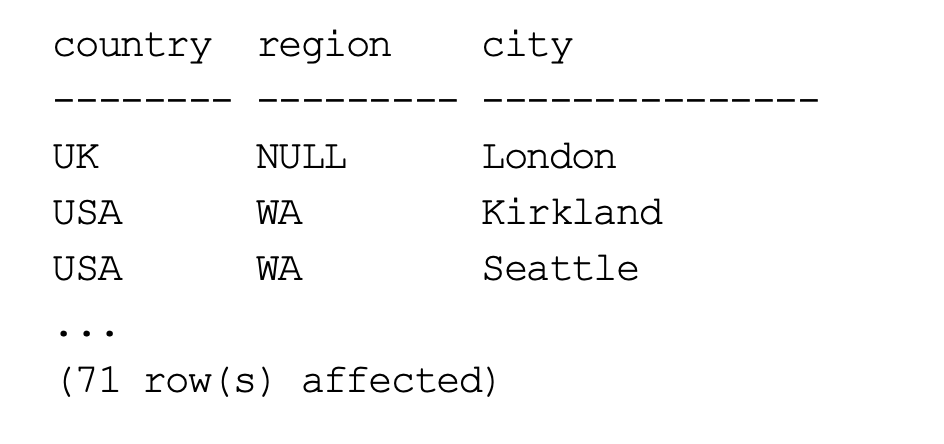
\includegraphics[width=0.9\textwidth]{img/examp1.png}
	\end{center}
	\captionsetup{justification=centering}
\end{figure}

Если вы хотите сохранить дубликаты, например, чтобы позже сгруппировать строки и подсчитать количество вхождений, то вместо оператора UNION следует использовать оператор UNION ALL. Оператор UNION ALL объединяет результаты двух входных запросов, но не пытается удалить дубликаты.

\begin{figure}[h!]
	\begin{center}
		
\includegraphics[width=0.9\textwidth]{img/unionall.png}
	\end{center}
	\captionsetup{justification=centering}
\end{figure}


\begin{figure}[h!]
	\begin{center}
		
\includegraphics[width=0.9\textwidth]{img/warn.png}
	\end{center}
	\captionsetup{justification=centering}
\end{figure}


\subsection{Оператор INTERSECT}
Оператор INTERSECT возвращает только различные строки, общие для обоих наборов. Другими словами, если строка хотя бы один раз появляется в первом наборе и
хотя бы один раз — во втором, она появится один раз в результате оператора
INTERSECT.

\begin{figure}[h!]
	\begin{center}
		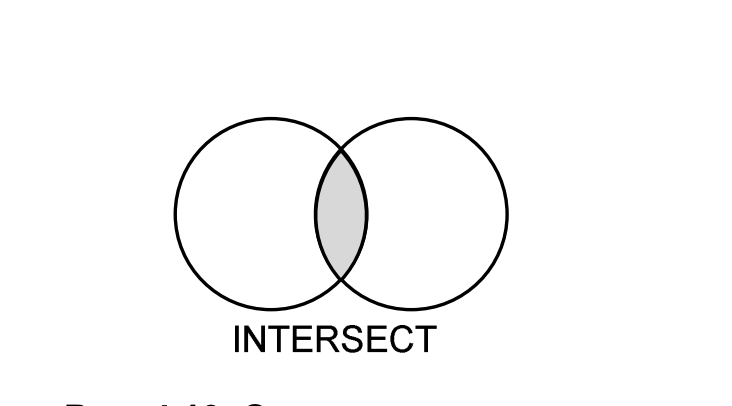
\includegraphics[width=0.5\textwidth]{img/intersect.png}
	\end{center}
	\captionsetup{justification=centering}
\end{figure}

\subsection{Оператор EXCEPT}
Оператор EXCEPT позволяет получить разность наборов данных. Он возвращает отличающиеся строки, которые появляются в первом запросе и не появляются во втором. Иными словами, если строка хотя бы раз появляется в первом запросе и ни
разу во втором, она один раз возвращается в выходном наборе.

\begin{figure}[h!]
	\begin{center}
		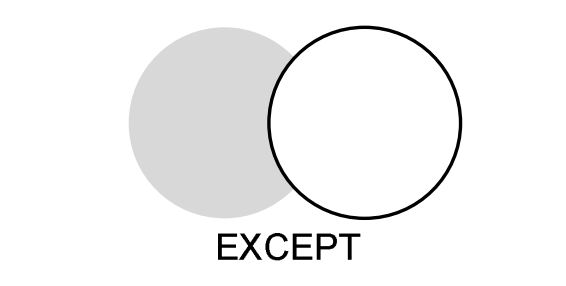
\includegraphics[width=0.5\textwidth]{img/except.png}
	\end{center}
	\captionsetup{justification=centering}
\end{figure}

Следующий запрос, который можно использовать в качестве примера использования оператора EXCEPT, возвращает местоположения сотрудников, не являющиеся
местоположениями клиентов

\begin{lstlisting}[label=lst:funcReturn, language=sql]
SELECT country, region, city
FROM HR.Employees
EXCEPT
SELECT country, region, city
FROM Sales.Customers;
\end{lstlisting}


\begin{figure}[h!]
	\begin{center}
		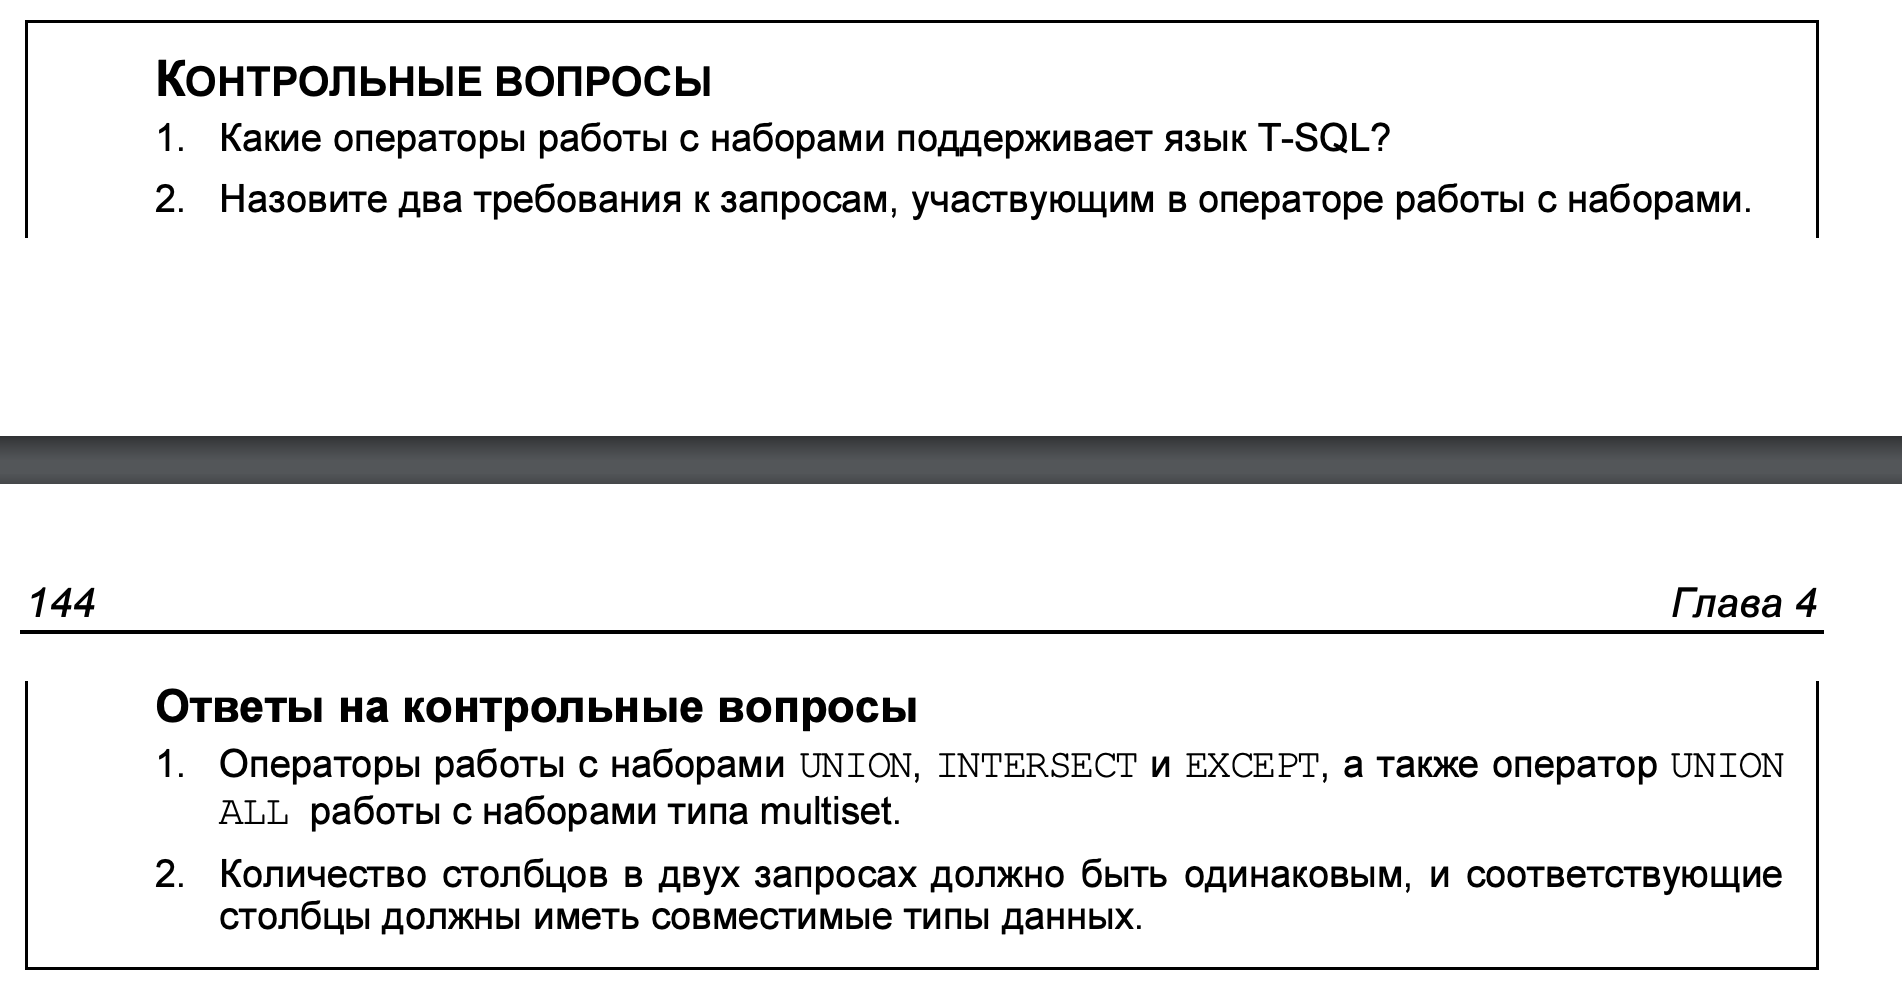
\includegraphics[width=0.9\textwidth]{img/control13.png}
	\end{center}
	\captionsetup{justification=centering}
\end{figure}



\subsection*{Резюме занятия}
\begin{itemize}
	\item Операторы работы с наборами сравнивают полные строки в результирующих
	наборах двух запросов. 
	\item  Оператор UNION объединяет входные наборы, возвращая несовпадающие строки. 
	\item Оператор UNION ALL объединяет входные наборы, не удаляя дубликаты. 
	\item Оператор UNION ALL объединяет входные наборы, не удаляя дубликаты. 
	\item Оператор EXCEPT возвращает строки, которые появляются в первом наборе, но не
	во втором, возвращая несовпадающие строки. 
\end{itemize}

\subsection*{Закрепление материала}

\begin{figure}[h!]
	\begin{center}
		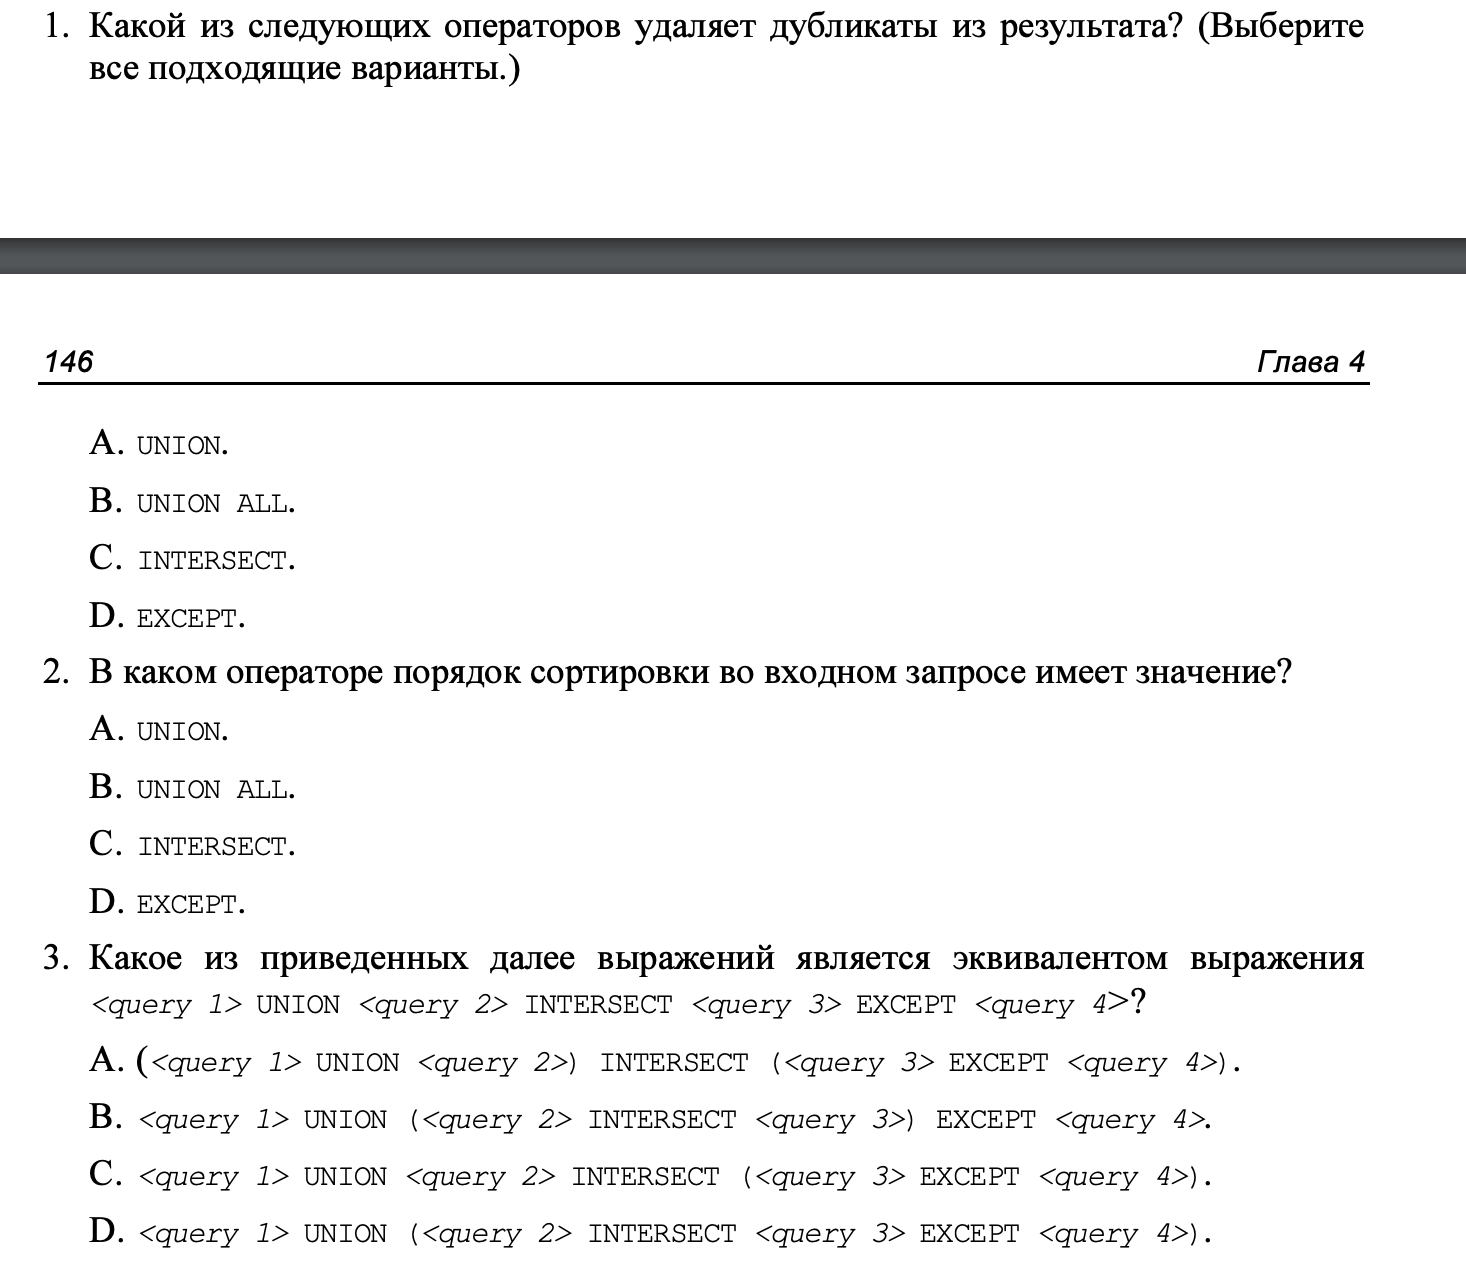
\includegraphics[width=0.9\textwidth]{img/zakrep10.png}
	\end{center}
	\captionsetup{justification=centering}
\end{figure}
\clearpage

\subsection*{Ответы}

\begin{figure}[h!]
	\begin{center}
		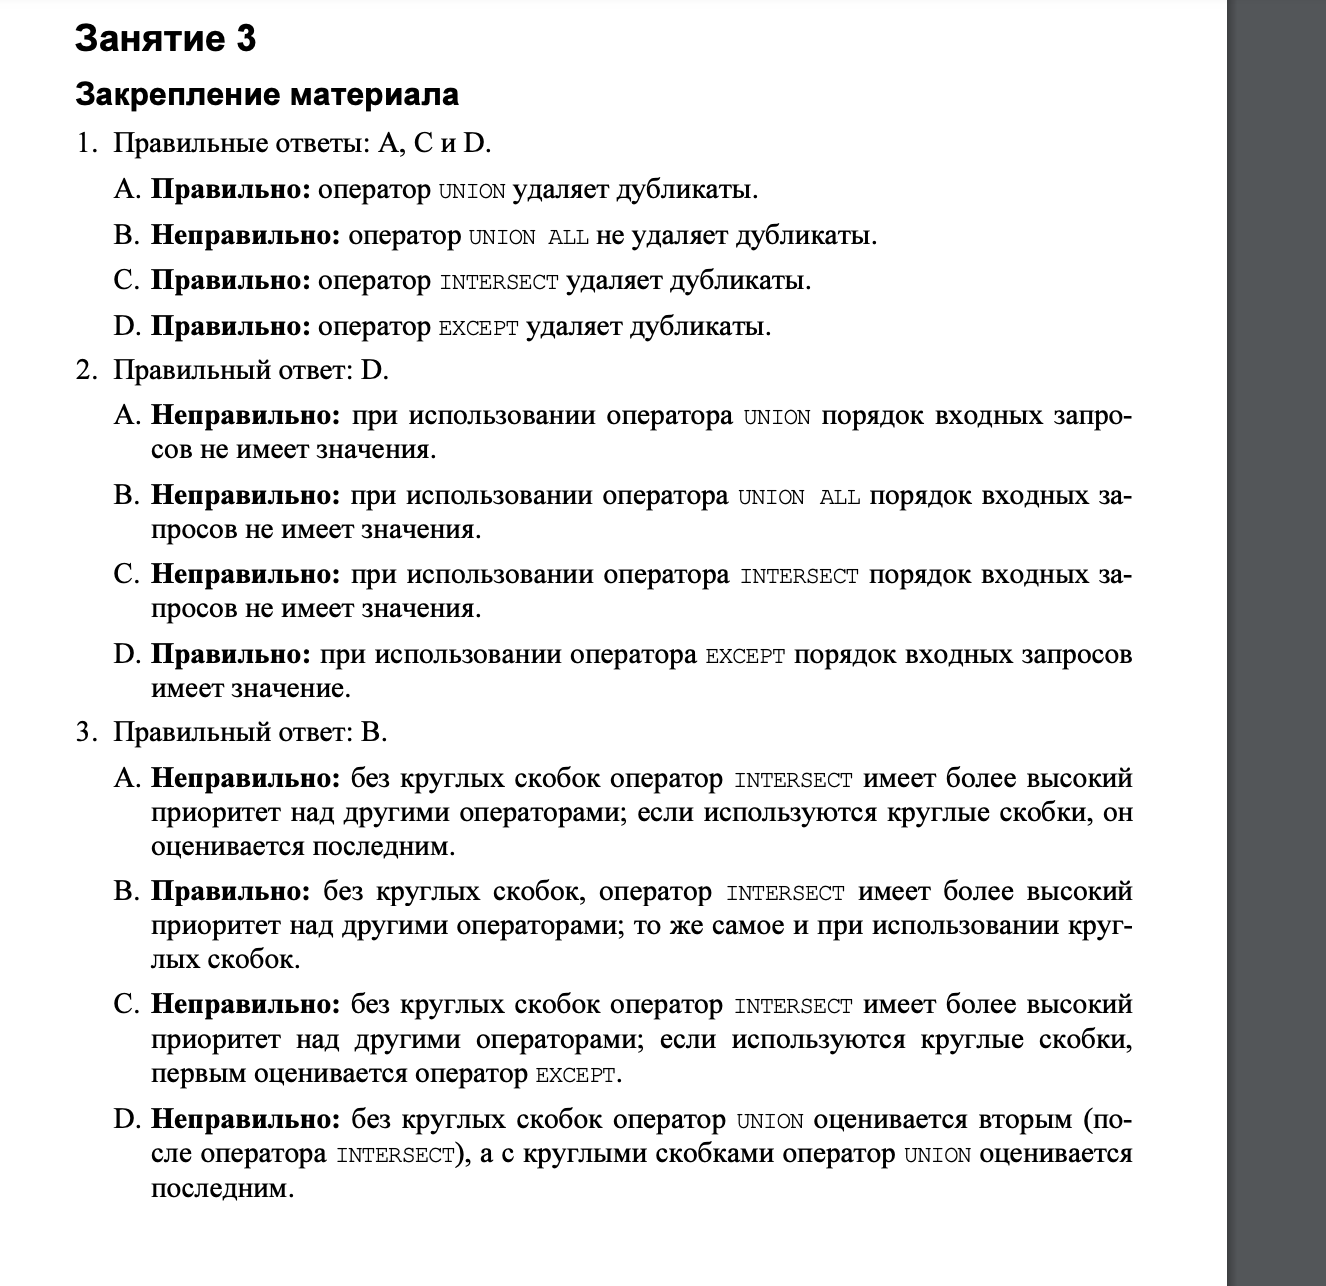
\includegraphics[width=0.8\textwidth]{img/ans10.png}
	\end{center}
	\captionsetup{justification=centering}
\end{figure}



\newpage
\subsection*{Упражнения}

\begin{figure}[h!]
	\begin{center}
		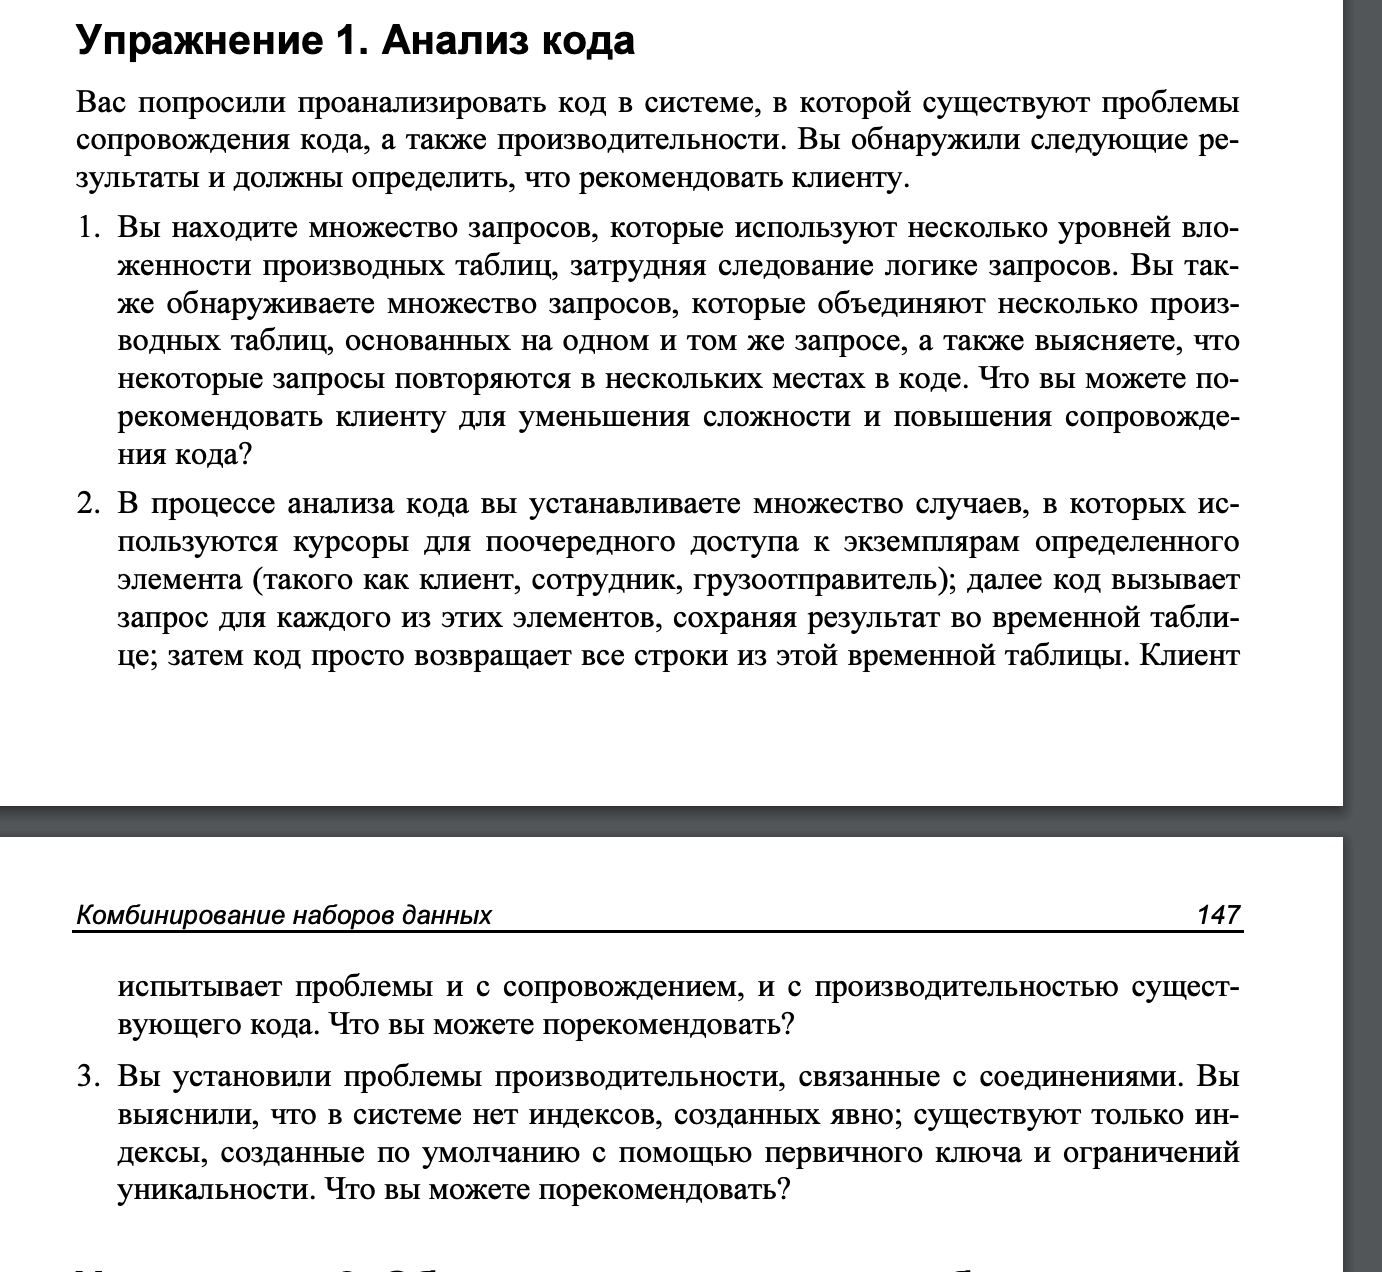
\includegraphics[width=0.9\textwidth]{img/ex11.png}
	\end{center}
	\captionsetup{justification=centering}
\end{figure}

\begin{figure}[h!]
	\begin{center}
		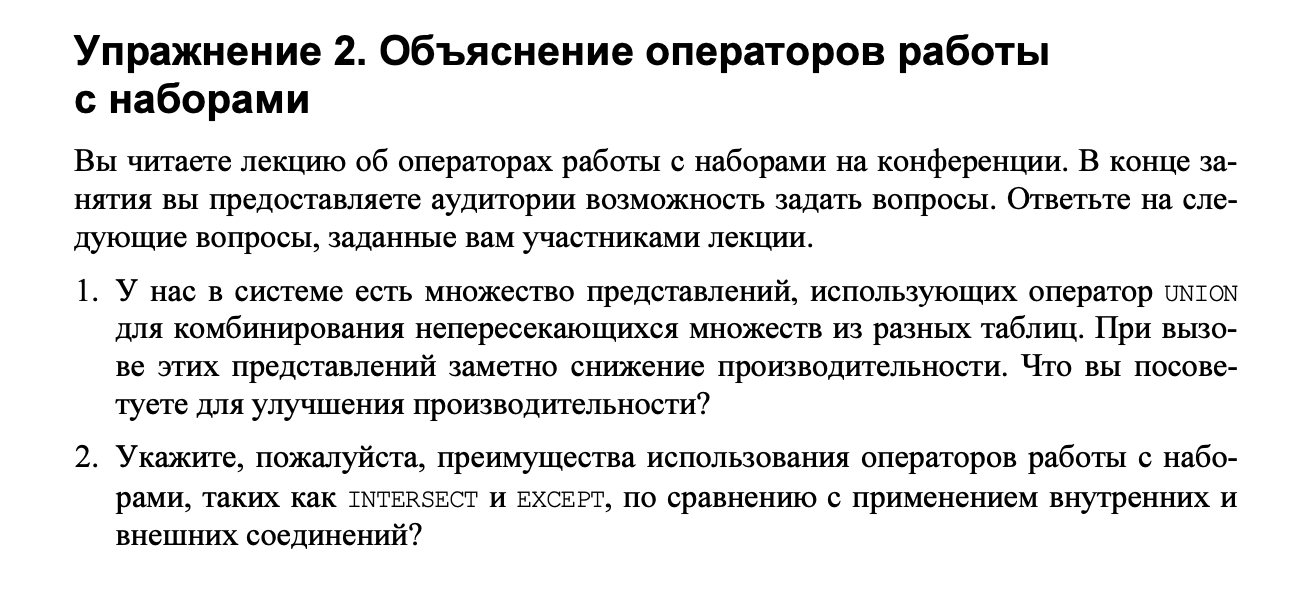
\includegraphics[width=0.9\textwidth]{img/ex12.png}
	\end{center}
	\captionsetup{justification=centering}
\end{figure}

\subsection*{Ответы}

\begin{figure}[h!]
	\begin{center}
		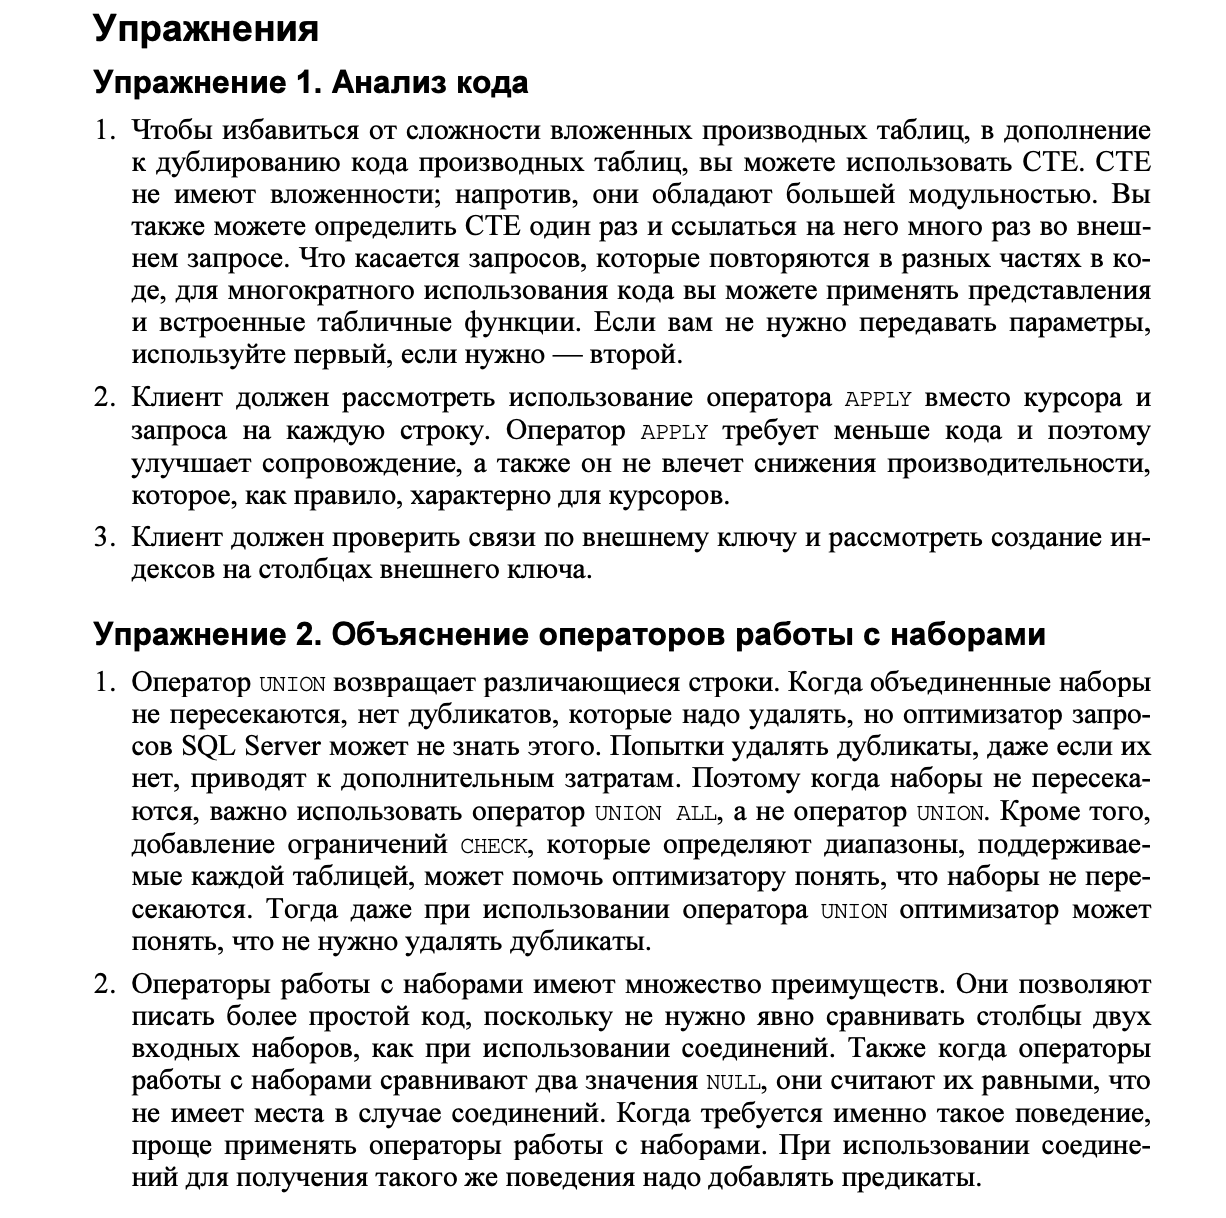
\includegraphics[width=0.9\textwidth]{img/eans4.png}
	\end{center}
	\captionsetup{justification=centering}
\end{figure}